\documentclass[a4paper,fleqn]{cas-sc}



\usepackage{amsmath,amssymb}
\usepackage{booktabs}
\usepackage{graphicx}
\usepackage{float}
\usepackage{siunitx}
\sisetup{round-mode=places, round-precision=3}
\usepackage[authoryear,round]{natbib}
\setcitestyle{aysep={, },citesep={; }}
\usepackage[all]{hypcap}
\usepackage{cleveref}
\crefname{appendix}{appendix}{appendices}
\Crefname{appendix}{Appendix}{Appendices}
\crefname{algocf}{algorithm}{algorithms}
\Crefname{algocf}{Algorithm}{Algorithms}

\usepackage[ruled,vlined,linesnumbered]{algorithm2e}
%\SetAlgoSkip{0pt}   % put once in preamble
\SetAlgoNoEnd
% Change only these lines to point the note at another rendered report.
\newcommand{\reportroot}{Journal_200patches_assets_oct21}
\newcommand{\datasetlabel}{HundredPatches/norm}
\newcommand{\distanceboxplot}{\reportroot/images/distance_profiles_box_whisker/no_shrinkage/distance_iqr_medians_rainy_multi_k3_box_whisker.png}
\newcommand{\nonrainydistanceboxplot}{\reportroot/images/distance_profiles_box_whisker/no_shrinkage/distance_iqr_medians_nonrainy_multi_k3_box_whisker.png}
\newcommand{\idwconfusionplot}{\reportroot/images/confusion_maps/IDW_confusion_map.png}
\newcommand{\ildwconfusionplot}{\reportroot/images/confusion_maps/ILDW_confusion_map.png}
\newcommand{\nonlinearconfusionplot}{\reportroot/images/confusion_maps/Nonlinear_Optimizer_confusion_map.png}
\newcommand{\patchgeometryplot}{\reportroot/images/patch_overview/patch_dimensions_scatter.png}
\newcommand{\patcheuropeoverview}{\reportroot/images/patch_overview/hundredpatches_europe_overview_basemap.png}
\newcommand{\taylorsummary}{\reportroot/images/taylor_200/combined_normalized.png}
\newcommand{\taylorsixpanel}{\reportroot/images/taylor_200/seasonal_clouds.png}
\newcommand{\tayloridw}{\reportroot/images/taylor_200/idw.png}
\newcommand{\taylorildw}{\reportroot/images/taylor_200/ildw.png}
\newcommand{\taylorsolverildw}{\reportroot/images/taylor_200/solverildw.png}
\newcommand{\taylorconvex}{\reportroot/images/taylor_200/convex_solver.png}
\newcommand{\taylorhomotopy}{\reportroot/images/taylor_200/homotopy_solver.png}
\newcommand{\taylorsolvergt}{\reportroot/images/taylor_200/solvergt.png}
\newcommand{\patchmetricboxplot}{\reportroot/images/summaries/patch_map_metrics_boxplots_readable_corr.png}
\newcommand{\linkhistplot}{\reportroot/images/patch_overview/link_count_histogram.png}
\newcommand{\largestpatchbinsplot}{\reportroot/images/largest_patch_distance_bins/largest_patch_distance_bins_k3.png}
\newcommand{\contextroot}{\reportroot/images/rain_patch_explorer_maps}
\newcommand{\contextvone}{\reportroot/images/rain_patch_explorer_maps/v1}
\newcommand{\contextvtwo}{\reportroot/images/rain_patch_explorer_maps/v2}
\newcommand{\contextscreenshotorigone}{\contextvone/202301280900_patch000_map.png}
\newcommand{\contextscreenshotorigtwo}{\contextvone/202301310900_patch000_map.png}
\newcommand{\contextscreenshotone}{\contextvtwo/RAD_OPERA_HOURLY_RAINFALL_ACCUMULATION_202301282100_patch000.png}
\newcommand{\contextscreenshottwo}{\contextvtwo/RAD_OPERA_HOURLY_RAINFALL_ACCUMULATION_202301310200_patch000.png}
\newcommand{\contextscreenshotthree}{\contextvone/202301311600_patch000_map.png}
\newcommand{\combinedcaseorigone}{\reportroot/images/patch_error_maps/combined/RAD_OPERA_HOURLY_RAINFALL_ACCUMULATION_202301280900_patch000.png}
\newcommand{\gtconvexcaseone}{\reportroot/images/case_studies/new_pattern_one/RAD_OPERA_HOURLY_RAINFALL_ACCUMULATION_202301280900_patch000.png}
\newcommand{\jgtcaseone}{\reportroot/images/j_behavior/gt_vs_convex_pattern_one/case1-gt-iterations.png}
\newcommand{\jconvexcaseone}{\reportroot/images/j_behavior/gt_vs_convex_pattern_one/case1-convex-iterations.png}
\newcommand{\gtconvexcasetwo}{\reportroot/images/case_studies/new_pattern_one/RAD_OPERA_HOURLY_RAINFALL_ACCUMULATION_202301310900_patch000.png}
\newcommand{\jgtcasetwo}{\reportroot/images/j_behavior/gt_vs_convex_pattern_one/case2-gt-iterations.png}
\newcommand{\jconvexcasetwo}{\reportroot/images/j_behavior/gt_vs_convex_pattern_one/case2-convex-iterations.png}
\newcommand{\combinedcaseorigtwo}{\reportroot/images/patch_error_maps/combined/RAD_OPERA_HOURLY_RAINFALL_ACCUMULATION_202301310900_patch000.png}
\newcommand{\combinedcaseone}{\reportroot/images/patch_error_maps/combined/RAD_OPERA_HOURLY_RAINFALL_ACCUMULATION_202301282100_patch000.png}
\newcommand{\combinedcasetwo}{\reportroot/images/patch_error_maps/combined/RAD_OPERA_HOURLY_RAINFALL_ACCUMULATION_202301310200_patch000.png}
\newcommand{\combinedcasethree}{\reportroot/images/patch_error_maps/combined/RAD_OPERA_HOURLY_RAINFALL_ACCUMULATION_202301311600_patch000.png}
\newcommand{\idwcaseorigone}{\reportroot/images/patch_error_maps/IDW/RAD_OPERA_HOURLY_RAINFALL_ACCUMULATION_202301280900_patch000_rainy.png}
\newcommand{\ildwcaseorigone}{\reportroot/images/patch_error_maps/ILDW/RAD_OPERA_HOURLY_RAINFALL_ACCUMULATION_202301280900_patch000_rainy.png}
\newcommand{\optcaseorigone}{\reportroot/images/patch_error_maps/OPT_NORM_ILDW_MULT_ILDW_INIT/RAD_OPERA_HOURLY_RAINFALL_ACCUMULATION_202301280900_patch000_rainy.png}
\newcommand{\idwcaseorigtwo}{\reportroot/images/patch_error_maps/IDW/RAD_OPERA_HOURLY_RAINFALL_ACCUMULATION_202301310900_patch000_rainy.png}
\newcommand{\ildwcaseorigtwo}{\reportroot/images/patch_error_maps/ILDW/RAD_OPERA_HOURLY_RAINFALL_ACCUMULATION_202301310900_patch000_rainy.png}
\newcommand{\optcaseorigtwo}{\reportroot/images/patch_error_maps/OPT_NORM_ILDW_MULT_ILDW_INIT/RAD_OPERA_HOURLY_RAINFALL_ACCUMULATION_202301310900_patch000_rainy.png}
\newcommand{\idwcaseone}{\reportroot/images/patch_error_maps/IDW/RAD_OPERA_HOURLY_RAINFALL_ACCUMULATION_202301282100_patch000_rainy.png}
\newcommand{\ildwcaseone}{\reportroot/images/patch_error_maps/ILDW/RAD_OPERA_HOURLY_RAINFALL_ACCUMULATION_202301282100_patch000_rainy.png}
\newcommand{\optcaseone}{\reportroot/images/patch_error_maps/OPT_NORM_ILDW_MULT_ILDW_INIT/RAD_OPERA_HOURLY_RAINFALL_ACCUMULATION_202301282100_patch000_rainy.png}
\newcommand{\idwcasetwo}{\reportroot/images/patch_error_maps/IDW/RAD_OPERA_HOURLY_RAINFALL_ACCUMULATION_202301310200_patch000_rainy.png}
\newcommand{\ildwcasetwo}{\reportroot/images/patch_error_maps/ILDW/RAD_OPERA_HOURLY_RAINFALL_ACCUMULATION_202301310200_patch000_rainy.png}
\newcommand{\optcasetwo}{\reportroot/images/patch_error_maps/OPT_NORM_ILDW_MULT_ILDW_INIT/RAD_OPERA_HOURLY_RAINFALL_ACCUMULATION_202301310200_patch000_rainy.png}
\newcommand{\idwcasethree}{\reportroot/images/patch_error_maps/IDW/RAD_OPERA_HOURLY_RAINFALL_ACCUMULATION_202301311600_patch000_rainy.png}
\newcommand{\ildwcasethree}{\reportroot/images/patch_error_maps/ILDW/RAD_OPERA_HOURLY_RAINFALL_ACCUMULATION_202301311600_patch000_rainy.png}
\newcommand{\optcasethree}{\reportroot/images/patch_error_maps/OPT_NORM_ILDW_MULT_ILDW_INIT/RAD_OPERA_HOURLY_RAINFALL_ACCUMULATION_202301311600_patch000_rainy.png}
\newcommand{\jcaseorigone}{\reportroot/images/j_behavior/opt_norm_ildw_mult_ildw_init/RAD_OPERA_HOURLY_RAINFALL_ACCUMULATION_202301280900_patch000.png}
\newcommand{\jcaseorigtwo}{\reportroot/images/j_behavior/opt_norm_ildw_mult_ildw_init/RAD_OPERA_HOURLY_RAINFALL_ACCUMULATION_202301310900_patch000.png}
\newcommand{\jcaseone}{\reportroot/images/j_behavior/opt_norm_ildw_mult_ildw_init/RAD_OPERA_HOURLY_RAINFALL_ACCUMULATION_202301282100_patch000.png}
\newcommand{\jcasetwo}{\reportroot/images/j_behavior/opt_norm_ildw_mult_ildw_init/RAD_OPERA_HOURLY_RAINFALL_ACCUMULATION_202301310200_patch000.png}
\newcommand{\jcasethree}{\reportroot/images/j_behavior/opt_norm_ildw_mult_ildw_init/RAD_OPERA_HOURLY_RAINFALL_ACCUMULATION_202301311600_patch000.png}

% Case-study panels use solver outputs with zero shrinkage.
\renewcommand{\gtconvexcaseone}{\reportroot/images/case_studies/no_shrinkage/RAD_OPERA_HOURLY_RAINFALL_ACCUMULATION_202301280900_patch000.png}
\renewcommand{\jgtcaseone}{\reportroot/images/j_behavior/no_shrinkage/case1-gt-iterations.png}
\renewcommand{\jconvexcaseone}{\reportroot/images/j_behavior/no_shrinkage/case1-convex-iterations.png}
\renewcommand{\gtconvexcasetwo}{\reportroot/images/case_studies/no_shrinkage/RAD_OPERA_HOURLY_RAINFALL_ACCUMULATION_202301310900_patch000.png}
\renewcommand{\jgtcasetwo}{\reportroot/images/j_behavior/no_shrinkage/case2-gt-iterations.png}
\renewcommand{\jconvexcasetwo}{\reportroot/images/j_behavior/no_shrinkage/case2-convex-iterations.png}

\renewcommand{\taylorsixpanel}{\reportroot/images/taylor_200_noshrinkage/seasonal_clouds.png}

\newcommand{\notebox}[3]{%
  \begingroup
  \setlength{\fboxsep}{2pt}%
  \fcolorbox{#1}{#2}{\textsf{\footnotesize #3}}%
  \endgroup
}

\DeclareRobustCommand{\editnote}[1]{%
  \texorpdfstring{%
    \nobreak\hfill
    \mbox{\notebox{red!50!black}{red!10}{#1}}%
  }{}%
}

\DeclareRobustCommand{\inlinenote}[1]{%
  \mbox{\notebox{red!50!black}{red!10}{#1}}%
}

\newcommand{\editsection}[2]{\section[#1]{#1\editnote{#2}}}
\newcommand{\editsubsection}[2]{\subsection[#1]{#1\editnote{#2}}}


%algs
\DeclareRobustCommand{\IDW}{\textsc{idw}}
\DeclareRobustCommand{\ILDW}{\textsc{ildw}}
\DeclareRobustCommand{\solverILDW}{\textsc{solver(ildw)}}
\DeclareRobustCommand{\solverGT}{\textsc{solver(gt)}}
\DeclareRobustCommand{\solverConvex}{\textsc{convex solver}}
\DeclareRobustCommand{\solverHomotopy}{\textsc{homotopy solver}}
\DeclareRobustCommand{\ConvexSolver}{\solverConvex}
\DeclareRobustCommand{\Homotopy}{\solverHomotopy}
\DeclareRobustCommand{\LBFGSB}{\textsc{lbfgsb}}
\DeclareRobustCommand{\OPTILDW}{\solverILDW}

% Column labels and compact numeric notation.
\newcommand{\RMSE}{RMSE}
\newcommand{\Bias}{Bias}
\newcommand{\Pearson}{Pearson $r$}
\newcommand{\meanPixels}{mean pixels}
\newcommand{\pmv}[2]{#1\,$\pm$\,#2}


\begin{document}
\let\WriteBookmarks\relax
\def\floatpagepagefraction{1}
\def\textpagefraction{.001}

\shorttitle{Precipitation Estimation from Commercial Microwave Links}
\shortauthors{G. Even et al.}

\title[mode=title]{Discrete Learning Algorithms for Precipitation Estimation from Commercial Microwave Links}

\author[mpi]{Guy Even}
\ead{guyeven@mpi-inf.mpg.de}

\author[mpi]{Andreas Karrenbauer}
\ead{andreas.karrenbauer@mpi-inf.mpg.de}

\author[mpi]{Rex Lei}
\ead{rexlei@mpi-inf.mpg.de}

\author[tau]{Jonatan Ostrometzky}
\ead{jonatano@tauex.tau.ac.il}

\author[cologne]{Christian Sohler}
\ead{sohler@cs.uni-koeln.de}

\author[mpi]{Iv\'an Soto}
\ead{ivanalisv@gmail.com}

\affiliation[mpi]{organization={MPI for Informatics},
  city={Saarbr\"ucken},
  country={Germany}}

\affiliation[tau]{organization={School of Electrical Engineering, Tel-Aviv University},
  city={Tel Aviv},
  country={Israel}}

\affiliation[cologne]{organization={University of Cologne},
  city={Cologne},
  country={Germany}}

\begin{abstract}
  Commercial microwave links (CMLs) are part of the infrastructure of wireless networks. Their measured attenuations have been studied as an opportunistic source for monitoring spatiotemporal rainfall and other atmospheric phenomena. CML attenuation measurements can enhance the spatiotemporal accuracy and resolution of existing weather monitoring instruments. In addition, they serve as stand-alone weather monitoring devices in places where dedicated weather monitoring devices are scarce or do not exist.

  Current techniques for 2D rainfall map reconstruction usually reduce CML measurements to virtual rain gauges, namely point measurements, and rely on interpolation techniques such as inverse distance weighting or Kriging. While effective in many scenarios, these methods are suboptimal because they do not address the modeling error introduced when a path-integrated attenuation measurement is replaced by a single-point rain-intensity value.

  In this study, we revisit the rainfall map reconstruction problem from CML signal attenuation measurements with a principled optimization approach. We formulate the problem of partial-to-complete field reconstruction as a physics-informed optimization problem. The reconstructed rainfall field is quantized and represented by pixel rainfall variables whose values are constrained to agree with the observed CML signal attenuations. The resulting solution minimizes a weighted sum of attenuation errors along the links, spatial differences between neighboring pixels, and the total rainfall over the map.

  To evaluate our approach, we create a benchmark of 200 rainfall maps and CML configurations, comprising 100 winter and 100 summer patches. Rainfall maps are extracted from EURADCLIM by identifying rain events across diverse terrain types and precipitation patterns. The selected patches have side lengths between 50 and 94 km. CMLs are overlaid using a publicly available Netherlands dataset, and attenuations are computed using the ITU-R P.838 model.

  We then solve the inverse problem to reconstruct rainfall maps from attenuations and compare the results with inverse distance weighting. Overall, this study reframes rainfall reconstruction from opportunistic sensing networks as a well-posed inverse problem with an explicit objective function. The framework also provides interpretability benefits compared to purely data-driven approaches.
\end{abstract}

\begin{highlights}
  \item Rainfall reconstruction from CMLs is formulated as an explicit inverse optimization problem.
  \item A benchmark is built from EURADCLIM rain maps and synthetic link attenuations.
  \item The formulation preserves path geometry instead of collapsing links to point measurements.
\end{highlights}

\begin{keywords}
  Commercial microwave links \sep Rainfall estimation \sep Inverse problems \sep Optimization \sep Remote sensing
\end{keywords}

\maketitle

\section{Introduction}

Accurate rainfall estimation is a major tool used for accurate hydrology studies, weather prediction, flood forecasting, and urban drainage management. Reliable information on the spatial and temporal structure of precipitation is particularly important in urban and densely populated environments, where short-duration convective events may produce strong local gradients and rapid hydrological response. Conventional weather monitoring tools, primarily rain gauges and weather radars, provide valuable information but also have well-known limitations. Rain gauges offer direct point measurements, and are considered very accurate when properly installed, but their spatial density is often insufficient for resolving localized rainfall variability. Weather radars provide wide-area coverage, yet their estimates are not at ground level, and are prone to many uncertainties such as scattering, blockages, unaccounted vertical variability of rainfall, and limited near-ground representativeness.

Commercial microwave links (CMLs) offer a complementary source of rainfall information. These links are widely deployed as part of cellular telecommunication backhaul networks and continuously transmit electromagnetic signals between fixed antennas in a line-of-sight installments, nowadays at frequencies of 10 GHz to 90 GHz. During rainfall, raindrops affect the microwave radiation, causing measurable attenuation of the received signal. Since the frequencies range of operational links are sensitive to rain-induced attenuation \cite{ITU,gunn1954microwave,olsen1978rain}, the same infrastructure for communication was shown to also serve as an opportunistic environmental sensing network \cite{RemkoCountry2,chwala2019cml,fencl2015commercial}. As the CMLs are already deployed at large scale, often form dense networks in urban and suburban areas (especially in recent times, where dedicated CMLs networks for smart-city management are being deployed \cite{ostrometzky2024opportunistic,janco2022rain}, and are gaining attention as part of the integrated sensing and communication (ISAC) paradigm \cite{han2023potential}), they can provide near-ground measurements integrated along their paths, which span between tens of meters to several kilometers. Note that CMLs can be used in combination with satellite microwave links (SML) to further enhance their capabilities \cite{nebuloni2025review}. %Not sure we need the last sentence, it is for us to be able to shove a citation...

The physical basis for CML rainfall sensing is based on the attenuation of the signal that is caused by precipitation \cite{gunn1954microwave, olsen1978rain}, and is described by the ITU-R power-law relation\editnote{AK: We should cite the standard here, but which one is the right one?} between rain rate and specific attenuation. Given the frequency and polarization of a link, the rain-induced attenuation accumulated along the link can be modeled as the path integral of the specific attenuation over the rainfall field. Thus, unlike a rain gauge, which measures rainfall at a point, a CML provides a path-integrated measurement. This distinction is fundamental. A single link does not directly observe the rainfall value at one location; rather, it constrains the average attenuation, and hence the rainfall intensity, along its propagation path. Consequently, rainfall reconstruction from CMLs is an inverse problem: the objective is to estimate a spatial rainfall field from a collection of line-integral-like measurements.

Many practical CML-based reconstruction methods simplify this inverse problem by first converting each link measurement into a single representative rain-rate value, often interpreted as a virtual rain gauge located at the link midpoint or at an assumed other point along the link path. Standard spatial interpolation techniques can then be applied to these virtual point observations. This approach is simple, computationally efficient, and often useful in practice. However, it also discards part of the geometric information contained in the link measurement. In particular, the fact that the attenuation is accumulated along an extended path is replaced by a point approximation. This simplification may introduce modeling errors, especially in heterogeneous rainfall fields or in regions where the geometry and density of the link network strongly influence the information available for reconstruction \cite{gat2019comparative,Leijnse2008}. %TODO: Add some references about paths

A more faithful treatment of CML data should account for the coupling between the unknown rainfall field and the measured attenuation along each link path. This coupling depends on the link geometry, length, frequency, polarization, and the spatial distribution of rain along the path. Reconstruction methods that explicitly incorporate this structure have the potential to use the available information more effectively, but they also lead to more challenging estimation problems. In particular, because the attenuation--rain-rate relation is nonlinear, the corresponding inverse problem may be formulated as a constrained nonconvex optimization problem over the rainfall field.

Evaluating such reconstruction methods is difficult in real operational settings because the true rainfall field is generally unknown. Real CML measurements also include additional effects that complicate the analysis, such as wet-antenna attenuation, baseline drift, quantization, hardware-dependent sampling, and measurement noise. While these effects are essential in operational systems, they make it difficult to isolate the intrinsic performance of the reconstruction algorithm itself. A controlled benchmark, in which the ground-truth rainfall field is known and the corresponding CML attenuations are generated through a forward physical model, provides a useful way to study this core inverse problem.

In this paper, we introduce such a benchmark framework. Starting from hourly EURADCLIM rainfall maps, we construct synthetic but physically grounded rain-event patches and generate corresponding noise-free CML attenuation measurements using the ITU-R forward model. This creates a controlled evaluation setting in which different reconstruction algorithms can be compared directly against the known rainfall field. By removing confounding measurement artifacts while preserving realistic spatial rainfall patterns, the proposed benchmark isolates the reconstruction problem and enables systematic analysis of the role of link geometry, interpolation assumptions, and optimization-based estimation.

We use this framework to compare standard inverse-distance weighting (IDW), a link-aware extension tailored to CML measurements, and a nonconvex optimization formulation that directly couples the estimated rainfall field to the measured attenuations.\editnote{AK: We should cite something for the other two methods} In addition, we analyze reconstruction quality as a function of distance from the available links, thereby quantifying how the spatial arrangement of the CML network affects estimation accuracy.

\subsection{Contributions}
\begin{enumerate}
  \item Introduction of a methodology for generating rain-event benchmarks for evaluation of rainfall estimation based on noise-free CML attenuation.
  \item Creation of a 200-patch benchmark comprising 100 winter and 100 summer patches.
  \item Introduction of a new algorithm ILDW - version of IDW tailored for CML's.
  \item Introduction of rain-rate estimation as a nonconvex constrained optimization problem. Improve coupling between the estimation and measured attenuation.
  \item Systematic evaluation of IDW, ILDW, and nonconvex optimization algorithms.
  \item Evidence of quality of estimates as a function of distance from links.

\end{enumerate}
%%%%%%%%%%%%%%%%%%%%%%%%%%%%%%%%%%%%%%%%%%%%%%%%%%%%%
\section{Background and Related Work}
\subsection{ITU-R Forward Model: Rain-Induced Attenuation }

During a rain event, the signal along a commercial microwave link experiences attenuation because raindrops absorb and scatter electromagnetic energy.
We use Recommendation ITU-R P.838-3 for converting rain-rate into specific attenuation~\citep{ITU}. The ITU-R model relates the rain rate $R$ (in \si{\milli\meter\per\hour})
to the \emph{specific attenuation} $\gamma_R$ (in \si{\deci\bel\per\kilo\meter}) through the power law
\begin{equation}\label{eq:ITU}
  \gamma_R = \kappa R^{\alpha},
\end{equation}
where the coefficients $\kappa$ and $\alpha$ depend on the link frequency and polarization \citep{ITU}. See Table~\ref{tab:itu_coeffs} for the coefficient values and resulting attenuation for horizontal polarization and rain rates of $1$--$8$ \si{\milli\meter\per\hour}.

The total rain-induced attenuation is the integral of $\gamma_R$ along the link. Thus, longer links accumulate more attenuation, and links operating at different frequencies or polarizations respond differently to the same rainfall field.
For a horizontal terrestrial link of length $L$ with uniform rain rate $R$ along the path, the total rain-induced attenuation is therefore $A=\gamma_R \cdot L$.
If the rain-rate field is discretized into pixels, the total rain-induced attenuation is the sum of the attenuations over the segments obtained by intersecting the link with the pixels it traverses.


%%%
\begin{table}[t]
  \centering
  \caption{ITU-R P.838-3 coefficients for horizontal polarization and resulting specific attenuation $\gamma_R$ for selected rain rates (\si{\milli\meter\per\hour}).}
  \label{tab:itu_coeffs}
  \begin{tabular}{
      S[table-format=2.0, round-mode=places, round-precision=0]
      S[table-format=1.5]
      S[table-format=1.3]
      S[table-format=1.3]
      S[table-format=1.3]
      S[table-format=1.3]
      S[table-format=1.3]
    }
    \hline
    \multicolumn{1}{c}{$f$}                            &
    \multicolumn{1}{c}{$\kappa_H$}                     &
    \multicolumn{1}{c}{$\alpha_H$}                     &
    \multicolumn{1}{c}{$\gamma_R(R=1)$}                &
    \multicolumn{1}{c}{$\gamma_R(R=2)$}                &
    \multicolumn{1}{c}{$\gamma_R(R=4)$}                &
    \multicolumn{1}{c}{$\gamma_R(R=8)$}                                                                               \\
    \multicolumn{1}{c}{(\si{\giga\hertz})}             &
    \multicolumn{1}{c}{}                               &
    \multicolumn{1}{c}{}                               &
    \multicolumn{1}{c}{(\si{\decibel\per\kilo\meter})} &
    \multicolumn{1}{c}{(\si{\decibel\per\kilo\meter})} &
    \multicolumn{1}{c}{(\si{\decibel\per\kilo\meter})} &
    \multicolumn{1}{c}{(\si{\decibel\per\kilo\meter})}                                                                \\
    \hline
    10                                                 & 0.01217 & 1.257  & 0.01217 & 0.0290861 & 0.069515 & 0.166140 \\
    15                                                 & 0.04481 & 1.1233 & 0.04481 & 0.0976162 & 0.212652 & 0.463251 \\
    20                                                 & 0.09164 & 1.0568 & 0.09164 & 0.1906398 & 0.396590 & 0.825032 \\
    25                                                 & 0.1571  & 0.9991 & 0.1571  & 0.3140041 & 0.627616 & 1.254450 \\
    30                                                 & 0.2403  & 0.9485 & 0.2403  & 0.4637466 & 0.894968 & 1.727168 \\
    40                                                 & 0.4431  & 0.8673 & 0.4431  & 0.8083232 & 1.474580 & 2.689996 \\
    \hline
  \end{tabular}
\end{table}
%%%

%%%%%%%%%%%%%%%%%%%%%%%%%%%%%%%%%%%%%%%%%%%%%%%%%%%%%
\section{Benchmark Construction\editnote{GE:stable}}
In this section, we describe how we constructed our benchmark of rain-event patches combined with CML rain-attenuation.  The resulting benchmark instances combine realistically derived rainfall maps with real-world link configurations, from which noise-free rain-induced attenuation measurements are generated for every link.
\subsection{Data Source}
We extract rain events from the European climatological gauge-adjusted radar precipitation dataset EURADCLIM \citep{overeem2023euradclim}. EURADCLIM is derived from OPERA European radar composites and provides hourly precipitation fields at 2 \si{\kilo\meter} spatial resolution over a large fraction of Europe. The dataset are distributed in HDF5 format according to the OPERA Data Information Model (ODIM) convention \citep{odimh5}. File-level access and documentation are provided through the KNMI data platform \citep{knmi_euradclim_project}.

\subsection{Automatic Extraction of Rain Events}
Each hourly EURADCLIM map is processed independently. We first average the rainfall field over a $4 \times 4$ window of native 2 \si{\kilo\meter} pixels, then retain the pixels whose smoothed rain rate is at least 3 \si{\milli\meter\per\hour}. The retained pixels are partitioned into connected components under $8$-neighborhood connectivity. The event-selection criterion requires both side lengths of a component's axis-aligned bounding box to fall between 50 \si{\kilo\meter} and 95 \si{\kilo\meter}; in the resulting 200-patch benchmark, the observed side lengths range from 50 to 94 \si{\kilo\meter}. The accepted bounding box defines the extent of the benchmark patch, so patch dimensions follow the rain events themselves. Fixing a common patch size would instead require cropping the larger events or padding the smaller ones with dry area.


%The extraction procedure is:
%\begin{enumerate}
%\item Compute a local mean version of the rainfall field using a $4 \times 4$ uniform averaging window.
%\item Keep pixels whose smoothed rainfall exceeds a threshold of 3.0 mm.
%\item Partition the retained pixels into connected components.
%\item Keep only those components whose bounding boxes have side lengths between 50 km and 95 km.
%\end{enumerate}


\subsection{Refinement and Smoothing}
We refine and smooth each rain patch derived from EURADCLIM rainfall maps by subdividing each pixel into $16 \times 16$ subpixels (each $125 \times 125$ m$^2$), followed by Gaussian smoothing with $\sigma = 1$ in subpixel units.
The resulting rain patches are treated as the ground-truth rainfall field.

\subsection{CML Dataset}
CML metadata (including link locations, lengths, and frequencies) are obtained from the publicly available 4TU dataset~\citep{overeem2016cml} (we assumed horizontal polarization for all links). For each rainfall patch, the set of links is cropped to the patch extent and overlaid on the rainfall field. The ITU-R rain-attenuation model is then applied along each link path to compute the corresponding attenuation values.


\begin{table}[H]
  \centering
  \begin{tabular}{lrrrrr}
    \toprule
    Patch size (km) & \# links & 1-multiplicity & 2-multiplicity \\
    \midrule
    $50 \times 50$  & 939      & 99             & 420            \\
    $62 \times 60$  & 1254     & 128            & 563            \\
    $72 \times 70$  & 1507     & 157            & 675            \\
    \bottomrule
  \end{tabular}
  \caption{Representative link multiplicities for three patch dimensions.
    The multiplicity of a link is defined as the number of frequencies assigned to it.
    The second column reports the total number of link--frequency pairs.
    In the data set, link multiplicities were either 1 or 2, with approximately $10\%$ of links having multiplicity 1.
  }
  \label{tbl:4TU link multiplicities}
\end{table}



\section{Benchmark Statistics}
In this section, we summarize key properties of the benchmark patches and their associated link geometry. We describe the geographic distribution and size range of the selected rain events, illustrate representative patch instances, summarize link statistics and topology, and report how rainy and dry pixels are distributed with respect to distance from the third-closest link.
%%%%%%%%%
%%%%%
%%
\paragraph{Patches.}
\begin{description}

  \item[Time.] The rain patches were extracted from hourly EURADCLIM maps between 18 and 31 January 2023 (winter) and from June 2023 (summer).

  \item[Geographic distribution.] See \Cref{fig:patches_europe_overview} for a depiction of the geographic locations of all 200 rain patches.

        \begin{figure}[!htbp]
          \centering
          \includegraphics[width=0.5\textwidth]{\patcheuropeoverview}
          \caption{Geographic locations of the 100 summer patches (red) and 100 winter patches (blue).}
          \label{fig:patches_europe_overview}
        \end{figure}

  \item[Patch sizes.]
        A scatter diagram of patch side lengths is depicted in \Cref{fig:patch scatter}. The selected benchmark patches have side lengths ranging from $50$ to $94$ \si{\kilo\meter}.


        \begin{figure}[!htbp]
          \centering
          \includegraphics[width=0.50\textwidth]{\patchgeometryplot}
          \caption{Patch width versus patch height for all 200 benchmark patches: winter patches are blue and summer patches are red. The mean patch area is 280,649 pixels (SD 83,607; pixel side length $125$ m).}
          \label{fig:patch scatter}
        \end{figure}
\item[Patch statistics.]
\begin{table}[!htbp]\centering\small\begin{tabular}{lrrrrr}
\toprule Descriptor & Mean & SD & Min & Median & Max \\
\midrule
Wet fraction & 0.803 & 0.157 & 0.329 & 0.816 & 1.000 \\
Mean wet rain rate ($\mathrm{mm/h}$) & 4.49 & 1.61 & 2.39 & 3.99 & 9.97 \\
95th percentile wet rain rate ($\mathrm{mm/h}$) & 12.19 & 7.07 & 3.48 & 9.80 & 34.23 \\
Coefficient of variation, wet pixels & 0.783 & 0.317 & 0.180 & 0.745 & 1.720 \\
Area fraction above $5\,\mathrm{mm/h}$ & 0.190 & 0.104 & 0.000 & 0.190 & 0.470 \\
Relative gradient ($\mathrm{km}^{-1}$) & 0.277 & 0.138 & 0.053 & 0.274 & 0.768 \\
\bottomrule\end{tabular}
\caption{Rain-pattern descriptors across all 200 benchmark patches, summarized from one value per patch. Wet pixels have rain rate at least 0.6 mm/h. For each patch, the wet-pixel coefficient of variation (CV) is the standard deviation of wet-pixel rain rates divided by their mean.\newline Relative gradient is defined as follows. At each pixel, the local gradient magnitude is $\sqrt{g_x^2+g_y^2}$. Let $h=0.125$ km be the spacing between adjacent pixel centers. At an interior pixel $p$, $g_x(p)=\tfrac12\bigl[(R(p)-R(p_{\leftarrow}))/h+(R(p_{\rightarrow})-R(p))/h\bigr]$, averaging the slope from the left neighbor to $p$ and the slope from $p$ to its right neighbor. Similarly, $g_y(p)=\tfrac12\bigl[(R(p)-R(p_{\uparrow}))/h+(R(p_{\downarrow})-R(p))/h\bigr]$, using the pixel above and the pixel below. At an edge where a neighbor is missing, the available one-sided slope is used. Thus both components have units of $\mathrm{mm\,h^{-1}\,km^{-1}}$. Dividing their patch-average magnitude by the patch mean rain rate cancels the rain-rate unit, so the relative gradient reported in the table has units of $\mathrm{km^{-1}}$.}
\label{tab:patch_rain_patterns}
\end{table}

The table summarizes the six patch-level descriptors; their winter and summer distributions are shown in \Cref{fig:rain-pattern-histograms}.
  \item[Sample patches.] Sample rain-events from the benchmark are depicted in \Cref{fig:case_gt_convex_202301280900,fig:case_gt_convex_202301310900} together with their geographic location.
\end{description}
\begin{figure}[!htbp]
  \centering
  \editnote{IS: Don't remember if this what we wanted, adding two versions in case we decide to keep one}\par
  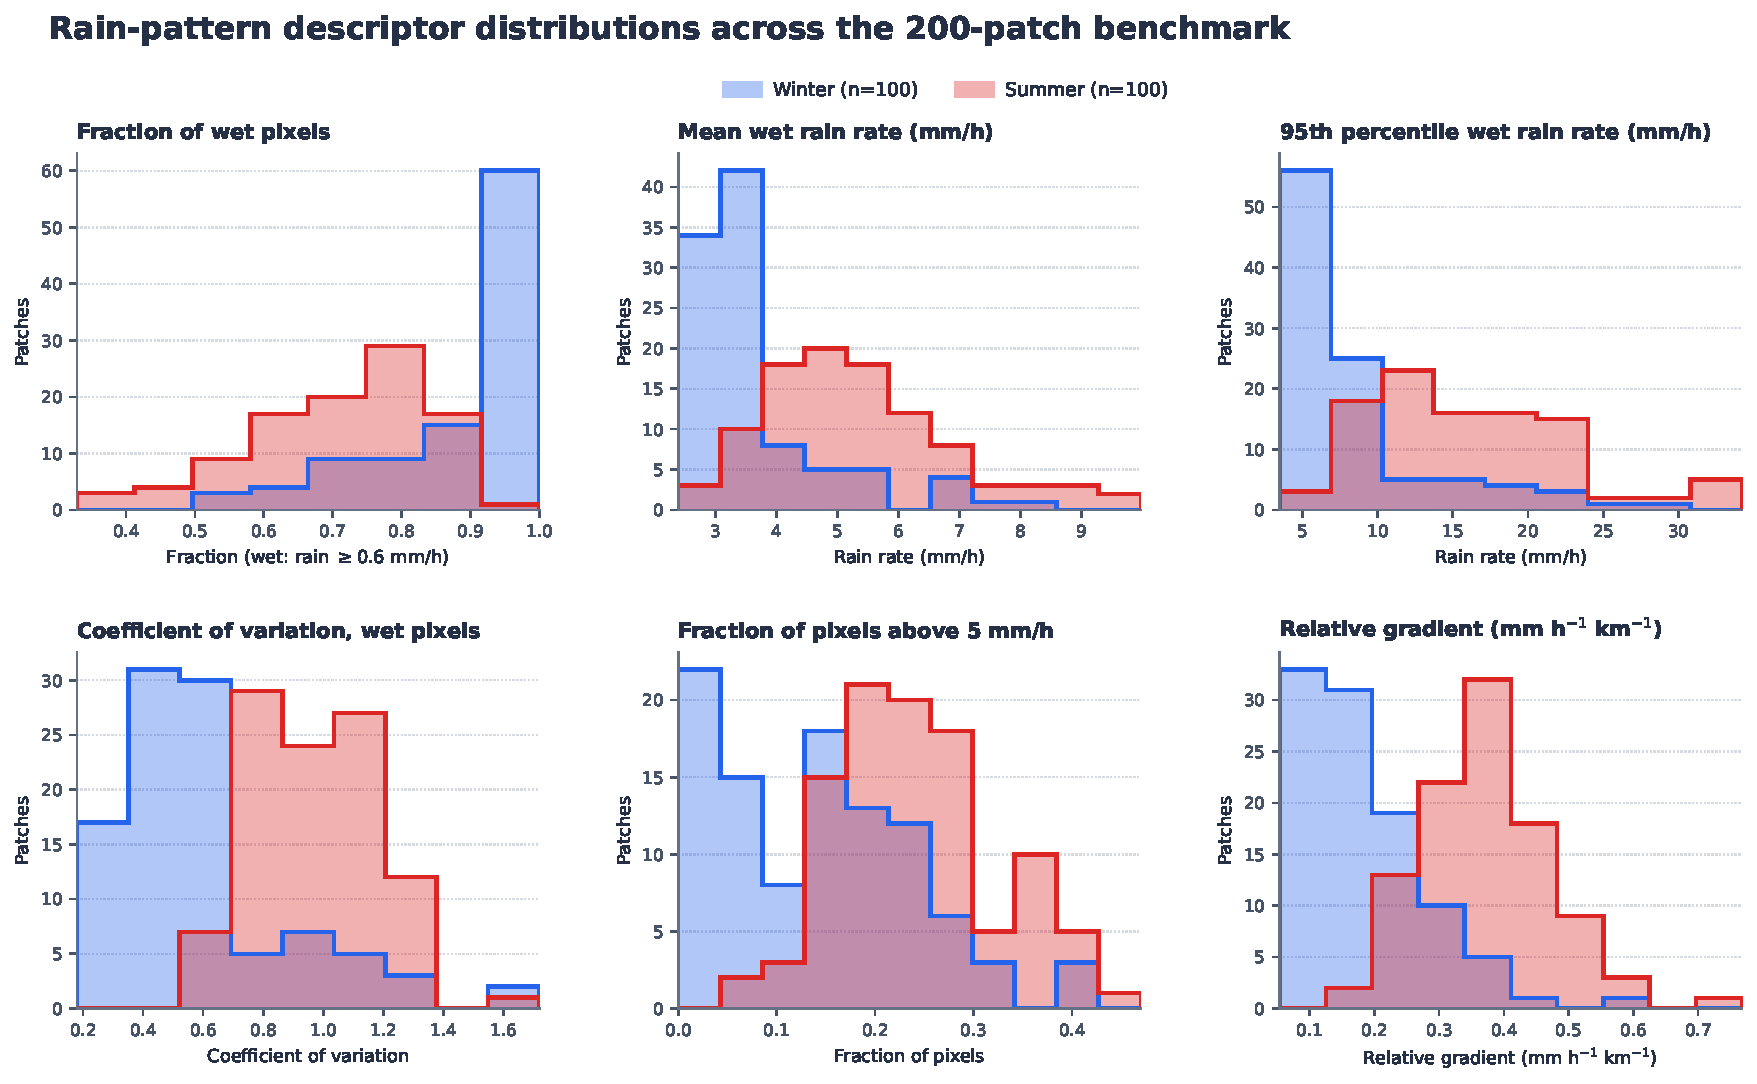
\includegraphics[width=\textwidth]{Journal_200patches_assets_oct21/images/rain_pattern_distributions_200/rain_pattern_histograms_200.pdf}
  \caption{Distributions of the six patch-level rain-pattern descriptors in Table~\ref{tab:patch_rain_patterns}, shown separately for the 100 winter and 100 summer benchmark patches. Wet pixels have rain rate at least $0.6$ mm/h. The coefficient of variation and relative gradient use the per-patch definitions given with the table.}
  \label{fig:rain-pattern-histograms}
\end{figure}
\begin{figure}[!htbp]
  \centering
  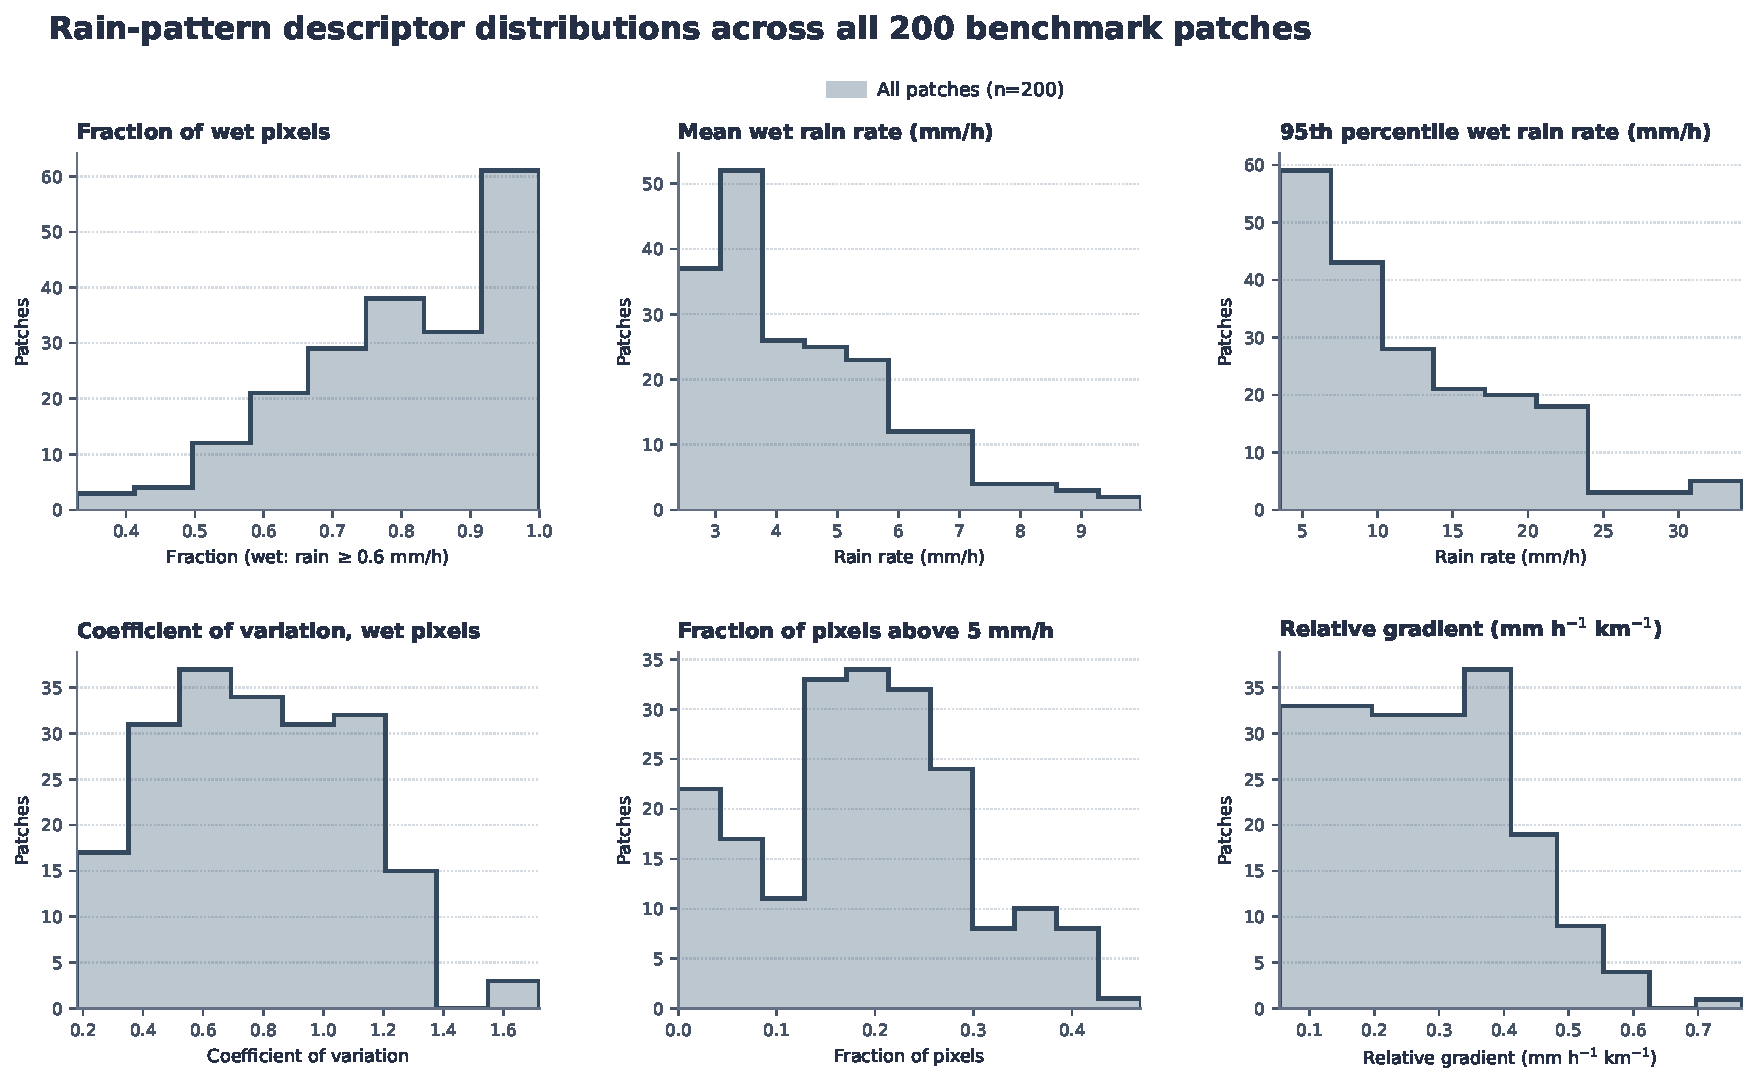
\includegraphics[width=\textwidth]{Journal_200patches_assets_oct21/images/rain_pattern_distributions_200/rain_pattern_histograms_200_combined.pdf}
  \caption{Distributions of the six patch-level rain-pattern descriptors in Table~\ref{tab:patch_rain_patterns}, pooled across all 200 benchmark patches. Wet pixels have rain rate at least $0.6$ mm/h. The coefficient of variation and relative gradient use the per-patch definitions given with the table.}
  \label{fig:rain-pattern-histograms-combined}
\end{figure}
%%%%%%%%%
%%%%%
%%

%%%%%%%%%
%%%%%
%%
\paragraph{Links.}
The largest patch overall by area is a summer patch from 19 June 2023 at 22:00, measuring $88\times 94$ \si{\kilo\meter}. Its link geometry appears in \Cref{fig:largest_patch_distance_bins}.
The pixels in this figure are binned according to their distance to the third-closest link. For a pixel $p$, let $d_3(p)$ denote the distance from the pixel center to the third-closest link. Equivalently, $d_3(p)$ is the smallest radius such that a disk centered at $p$ intersects at least three links.

\Cref{tab:largest_patch_distributions} summarizes link lengths, frequencies and endpoint degrees in this patch (endpoint degree is the number of link--frequency observations incident to the endpoint). See \Cref{tbl:4TU link multiplicities} for the number of links and their multiplicities for typical patch sizes (multiplicity 2 means a link operating at two frequencies).


\begin{figure}[t]
  \centering
  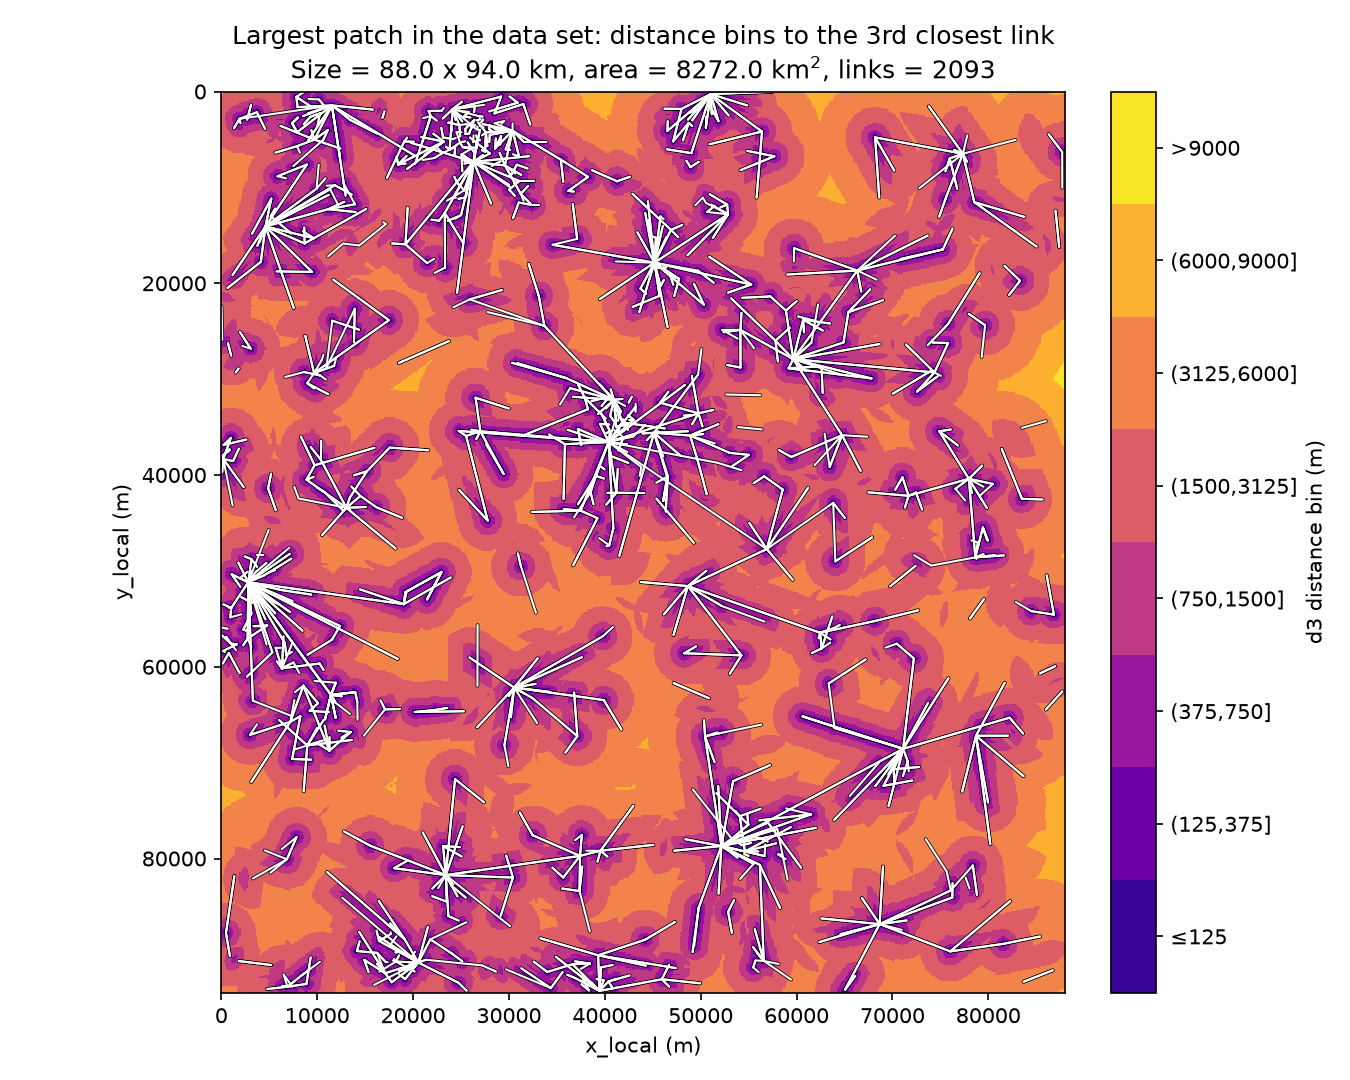
\includegraphics[width=0.88\textwidth]{Journal_200patches_assets_oct21/images/largest_patch_distance_bins/largest_patch_distance_bins_summer_largest_k3.png}
  \caption{$d_3$-bin map for the largest patch overall by area: the summer patch from 19 June 2023 at 22:00 ($88\times 94$ \si{\kilo\meter}). Each pixel is colored according to its distance bin, and the complete link geometry is overlaid in white.}

  \label{fig:largest_patch_distance_bins}
\end{figure}


\begin{table}[!htbp]
  \centering
  \begin{minipage}[t]{0.31\textwidth}
    \centering
    \scriptsize
    \begin{tabular}{lrr}
      \toprule
      Link length bin (km) & Count & \%   \\
      \midrule
      $[0,1)$         & 366   & 17.5 \\
      $[1,2)$         & 571   & 27.3 \\
      $[2,4)$         & 608   & 29.0 \\
      $[4,8)$         & 423   & 20.2 \\
      $[8,16)$        & 118   & 5.6  \\
      $[16,24]$       & 7     & 0.3  \\
      \bottomrule
    \end{tabular}
  \end{minipage}
  \hfill
  \begin{minipage}[t]{0.31\textwidth}
    \centering
    \scriptsize
    \begin{tabular}{lrr}
      \toprule
      Link frequency bin (GHz) & Count & \%   \\
      \midrule
      $[10,15)$           & 20    & 1.0  \\
      $[15,20)$           & 74    & 3.5  \\
      $[20,25)$           & 87    & 4.2  \\
      $[25,30)$           & 284   & 13.6 \\
      $[30,35)$           & 106   & 5.1  \\
      $[35,40)$           & 1433  & 68.5 \\
      $[40,60]$           & 89    & 4.3  \\
      \bottomrule
    \end{tabular}
  \end{minipage}
  \hfill
  \begin{minipage}[t]{0.31\textwidth}
    \centering
    \scriptsize
    \begin{tabular}{lrr}
      \toprule
      Link endpoint degree bin & Count & \%   \\
      \midrule
      $1$                 & 188   & 15.1 \\
      $2$                 & 617   & 49.7 \\
      $3,4$               & 268   & 21.6 \\
      $5,6$               & 78    & 6.3  \\
      $7..10$             & 45    & 3.6  \\
      $11..20$            & 28    & 2.3  \\
      $\geq 21$          & 18    & 1.4  \\
      \bottomrule
    \end{tabular}
  \end{minipage}
  \caption{Link statistics for the largest patch ($88\times 94$ \si{\kilo\meter}), which contains 2,093 links and 1,242 link endpoints. The tables give the binned distributions, as counts and percentages, of link length (left), link carrier frequency (middle), and endpoint degree (right). The degree of an endpoint is the number of links incident to it.}

  \label{tab:largest_patch_distributions}
\end{table}



\paragraph{Rainy/Dry Pixel Distance Stratification.}
We considered all 200 benchmark patches and classified the pixels in each patch as rainy or dry using a rainfall threshold of \SI[round-mode=none]{0.6}{\milli\meter\per\hour}.
Each of these two pixel sets was then partitioned into bins according to the pixel-level distance $d_3(p)$.
The mean and standard deviation of the rainy-pixel and dry-pixel counts in each distance bin, computed across all patches, are reported in \Cref{tab:rainy_nonrain_counts}.


\begin{table}[!htbp]\centering\small\setlength{\tabcolsep}{3pt}\begin{tabular*}{\textwidth}{@{\extracolsep{\fill}}lrrrrrr@{}}
\toprule & \multicolumn{3}{c}{Rainy pixels} & \multicolumn{3}{c}{Non-rainy pixels} \\
\cmidrule(lr){2-4}\cmidrule(lr){5-7}
$d_3$ bin (m) & Mean count & Mean \% & SD & Mean count & Mean \% & SD \\
\midrule
$\leq$125 & 3905.3 & 1.80 & 1067.8 & 1053.3 & 1.67 & 967.8 \\
(125,375] & 15353.2 & 7.05 & 4225.3 & 4183.0 & 6.60 & 3763.6 \\
(375,750] & 24845.0 & 11.29 & 7280.0 & 6401.2 & 10.26 & 5763.7 \\
(750,1500] & 48587.4 & 21.88 & 15505.5 & 12184.0 & 18.92 & 11231.5 \\
(1500,3125] & 83847.9 & 37.38 & 29719.7 & 20272.2 & 31.78 & 19209.7 \\
(3125,6000] & 42951.5 & 18.98 & 16795.7 & 11518.4 & 19.75 & 11019.5 \\
(6000,9000] & 3314.4 & 1.46 & 2567.1 & 1631.6 & 3.61 & 2045.8 \\
>9000 & 385.8 & 0.17 & 787.5 & 214.9 & 0.41 & 573.9 \\
\midrule Total & 223268.6 & 100 & 74239.5 & 57324.8 & 100 & 52090.6 \\
\bottomrule\end{tabular*}
\caption{Ground-truth rainy and non-rainy pixel counts by $d_3$ bin. Counts and within-class percentages are first computed per patch and then averaged across all 200 patches.}
\label{tab:rainy_nonrain_counts}
\end{table}

%%%%%%%%%%%%%%%%%%%%%%%%%%%%%%%%%%%%%%%%%%%%%%%%%%%%%
\section{Inverse Solvers: From Link Attenuations to Rainfall Maps\editnote{GE:stable}}
In this section, we present three solvers for the inverse problem: IDW, ILDW, and a nonconvex optimization model.

\subsection{Problem Formulation}
The inputs for the inverse problem consists of a set of links $\mathcal{L}$ in a patch $P$ (set of pixels). Every link $\ell$ has an attenuation $A_{\ell}$ and the following attributes: frequency, polarization, endpoints and length $|\ell|$.

The output is an estimated rain-rate field $\hat{R}:P\rightarrow \mathbb{R}_{\geq 0}$.

\subsection{Rain Equivalent for Link Attenuation}\label{sec:rain rate equivalent}
The \emph{rain-rate equivalent} $R_{\ell}$ of link $\ell$ is the uniform rain-rate along the link that would cause the link total attenuation $A_\ell$. This rain-rate is derived from the ITU-R model by:
\[
  R_\ell \triangleq \left(\frac{A_\ell/|\ell|}{\kappa_\ell}\right)^{1/\alpha_\ell}\;,
\]
where $(\kappa_\ell,\alpha_\ell)$ the ITU-R P.838-3 coefficients corresponding to the link's frequency and polarization.

\subsection{IDW}
Inverse-distance weighting (IDW) is one of the standard interpolation strategies used in commercial-microwave-link rainfall reconstruction
\citep{zimmerman1999experimental,jin2003comparison_krigbetter,chen2012estimation_idwforrain,chwala2019cml,eshel2020idw,eshel2021quantitative}.
The input consists of a set of links, where each link $\ell$ carries a total attenuation, frequency, and polarization.

IDW for CML's replaces every link $\ell$ with a virtual rain-gauge $g_{\ell}$ positioned at the midpoint between the endpoints of $\ell$. The rain-rate associated with $g_{\ell}$ is simply the rain-rate equivalent $R_{\ell}$. Inverse-distance weighting is applied with the virtual gauges positions and rain-rates as inputs.

We consider a setting in which the weight of a gauge decreases quadratically (i.e., decay exponent equals $2$) and the maximum radius of influence $r_{\max}$ is set to $15$ \si{\kilo\meter}. Distances to pixels are measured to the center of the pixel.
If one or more link midpoints lie inside pixel $p$, then the estimated rainfall in pixel $p$ is set to the mean of their rainfall estimates. The pseudocode for IDW appears in \Cref{alg:idw}.


\begin{algorithm}[H]
  \caption{Discretized IDW. Each link is replaced with a virtual gauge located at the midpoint of the link. The rain-rate at the gauge is set to the rain-rate equivalent of its link. IDW is then applied with respect to these virtual gauges. We set the exponent of the decay to $2$. }
  \label{alg:idw}
  \DontPrintSemicolon
  \KwData{link set $\mathcal{L}$, a patch $P$, and a maximum influence distance $r_{\max}$}
  \KwResult{rainfall field $\hat R:P\rightarrow\mathbb{R}_{\geq 0}$}
  \ForEach(\tcp*[f]{compute rain-rate equivalent per link}){link $\ell \in \mathcal{L}$}{%
    $(\ell.\kappa,\ell.\alpha) \gets \mathrm{ITU838}(\ell.\mathrm{freq},\ell.\mathrm{polarization})$\;
    $R_\ell\gets \left(\dfrac{A_\ell/|\ell|}{\ell.\kappa}\right)^{1/\ell.\alpha}$\;
  }
  \ForEach(\tcp*[f]{compute rain $\hat{R}(p)$}){pixel $p \in {P}$}{
    $M_p \gets \{\ell \in \mathcal{L} : \ell.\mathrm{midpoint} \in p\}$\;
    \eIf{$M_p \neq \emptyset$}{
      $\hat{R}(p) \gets \dfrac{1}{|M_p|}\sum_{\ell \in M_p} R_\ell$\tcp*[r]{pixel contains a link endpoint}
    }{
      $N_p \gets \{\ell \in \mathcal{L} : \|\ell.\mathrm{midpoint}-p.\mathrm{center}\|_2 \le r_{\max}\}$\;
      \eIf{$N_p = \emptyset$}{
        $\hat{R}(p) \gets 0$\tcp*[r]{pixel far from links}
      }{
        $\hat{R}(p) \gets \sum_{\ell \in N_p}\dfrac{\|\ell.\mathrm{midpoint}-p.\mathrm{center}\|_2^{-2}}{\sum_{\ell' \in N_p}\|\ell'.\mathrm{midpoint}-p.\mathrm{center}\|_2^{-2}} \cdot R_\ell$\;
      }
    }
  }
\end{algorithm}


\subsubsection{ILDW}
We propose a variation of IDW that alleviates the mismatch between measured link attenuation and attenuation computed from the IDW-estimated rainfall field.
We refer to this variation as inverse link-distance weighting (ILDW).
ILDW assigns a weight to every link that is inversely proportional to the distance between the pixel and the link, where
\[
  \operatorname{dist}(p,\ell) \triangleq \min_{q\in \ell} \|p.\textrm{center}-q\|\;.
\]

As in IDW, we set the decay exponent to $2$ and the maximum radius of influence $r_{\max}$ is set to $15$ \si{\kilo\meter}.
If one or more links cross the pixel, the estimated rain-rate is taken to be the mean of the corresponding link rain-rate equivalents. Otherwise, the estimate is a weighted average over links within distance $r_{\max}$ (set to 15km). The pseudocode for ILDW is shown in \Cref{alg:ildw}, with lines that differ from IDW highlighted in red.

\begin{algorithm}[H]
  \caption{Discretized ILDW. Rainfall is averaged by inverse squared distance to a link. Lines that are different from their corresponding lines in IDW are colored red. }
  \label{alg:ildw}
  \DontPrintSemicolon
  \KwData{link set $\mathcal{L}$, a patch $P$, and a maximum influence distance $r_{\max}$}
  \KwResult{rainfall field $\hat R:P\rightarrow\mathbb{R}_{\geq 0}$}
  \ForEach(\tcp*[f]{compute rain-rate equivalent per link}){link $\ell \in \mathcal{L}$}{%
    $(\ell.\kappa,\ell.\alpha) \gets \mathrm{ITU838}(\ell.\mathrm{freq},\ell.\mathrm{polarization})$\;
    $R_\ell\gets \left(\dfrac{A_\ell/|\ell|}{\ell.\kappa}\right)^{1/\ell.\alpha}$\;
  }
  \ForEach(\tcp*[f]{compute rain $\hat{R}(p)$}){pixel $p \in {P}$}{
    \textcolor{red}{$X_p \gets \{\ell \in \mathcal{L} : \ell\cap p \neq \emptyset\}$}\;
    \eIf{\textcolor{red}{$X_p$} $\neq \emptyset$}{
      \textcolor{red}{$\hat{R}(p) \gets \dfrac{1}{|X_p|}\sum_{\ell \in X_p} R_\ell$\tcp*[r]{at least one link traverses the pixel}
      }}{
      \textcolor{red}{$N_p \gets \{\ell \in \mathcal{L} : \mathrm{dist}(p,\ell) \le r_{\max}\}$}\;
      \eIf{$N_p = \emptyset$}{
        $\hat{R}(p) \gets 0$\tcp*[r]{pixel far from links}
      }{\textcolor{red}{
          $\hat{R}(p) \gets \sum_{\ell \in N_p}\dfrac{\mathrm{dist}^{-2}(p, \ell)}{\sum_{\ell' \in N_p}\mathrm{dist}^{-2}(p, \ell')} \cdot R_\ell$\;}
      }
    }
  }
\end{algorithm}

\newpage
\subsubsection{Nonconvex Formulation}

We formulate the inverse problem as a constrained optimization problem. The decision variables are the estimated rain-rates \(\hat{R}(p)\) for all pixels \(p \in P\). The constraints are simply nonnegativity constraints that reflect the physical requirement that rainfall is nonnegative. The objective is to minimize $J(\hat{R})$, where the cost function $J$ consists of the $4$ weighted terms:
\[
  J(\hat{R}) =
  w_{\mathrm{atten}} \cdot J_{\mathrm{atten}}(\hat{R})
  +
  w_{1d} \cdot J_{1d}(\hat{R})
  +
  w_{2d} \cdot J_{2d}(\hat{R})
  +
  w_{\mathrm{total}} \cdot J_{\mathrm{total}}(\hat{R})\;.
\]
The terms in $J(\hat{R})$ are as follows:
\begin{enumerate}
  \item The attenuation term $J_{\mathrm{atten}}$ quantifies disagreement between observed and estimated link attenuations.
        For a rain-rate field estimate $\hat{R}:P \rightarrow \mathbb{R}_{\geq 0}$ and a link $\ell$, let $A_{\ell}(\hat{R})$ denote the attenuation induced on $\ell$ by $\hat{R}$.
        This attenuation is computed using the ITU-R forward model with the link's frequency and polarization.
        The attenuation term $J_{\mathrm{atten}}$ is defined by
        \[
          J_{\mathrm{atten}}(\hat{R}) \triangleq
          \frac{1}{|\mathcal{L}|}
          \sum_{\ell \in \mathcal{L}}
          \frac{\bigl( A_\ell(\hat{R}) - A_\ell \bigr)^2}{|\ell|}\;.
        \]
  \item
        The first-difference term $J_{1d}$ enforces spatial smoothness, and is defined by
        \[
          J_{1d}(\hat{R}) \triangleq
          \frac{1}{|P|}
          \sum_{(u,v)\in\mathcal{E}(P)} (\hat{R}(u) - \hat{R}(v))^2\;,
        \]
        where $\mathcal{E}(P)$ is the set of horizontally and vertically adjacent pixel pairs in patch $P$.
  \item
        The second-difference term $J_{2d}$ penalizes curvature, and is defined by
        \[
          J_{2d}(\hat{R}) =
          \frac{1}{|P|}
          \sum_{(p,q,t)\in\mathcal{T}(P)} \bigl((\hat{R}(q) - \hat{R}(p)) - (\hat{R}(t) - \hat{R}(q))\bigr)^2,
        \]
        where $\mathcal{T}(P)$ is the set of horizontal and vertical triples of collinear pixels in patch $P$.
  \item
        The shrinkage term $J_{\mathrm{total}}$ biases the solution toward smaller overall rainfall values, and is defined by
        \[
          J_{\mathrm{total}}(\hat{R}) \triangleq
          \frac{1}{|P|}
          \sum_{p \in P} \hat{R}(p)^2.
        \]
\end{enumerate}

\paragraph{Implementation Details:}
\begin{enumerate}
  \item
        The weights of $J_{\mathrm{atten}}$, $J_{1d}$, and $J_{2d}$ are set to the reciprocals of their values evaluated at the ILDW solution, and we further divide $w_{2d}$ by $2$. For the no-shrinkage results reported here, we set $w_{\mathrm{total}}=0$, so the shrinkage term does not affect the solution. This normalizes the remaining objective terms instance-by-instance.
  \item
        We use the L-BFGS-B algorithm \citep{byrd1995limited,zhu1997algorithm}, a limited-memory quasi-Newton method for smooth constrained optimization, as implemented in SciPy \citep{scipy}.
\end{enumerate}

\paragraph{Nonconvex Cost Function:}
The ITU-R forward model (\Cref{eq:ITU}) attaches an attenuation exponent $\alpha$ to every link based on its frequency and polarization.
When $\alpha=1$, the predicted attenuation is linear in the rain-rate variables, so
$J_{\mathrm{atten}}$ is a sum of squares of linear residuals and is convex.
For $\alpha\neq 1$, the power-law attenuation makes the residual nonlinear,
and the attenuation term is generally nonconvex.
The nonconvexity emphasizes the importance of the initial solution used by the solver because local minima need not be global minima. We illustrate this nonconvexity with a concrete $3\times3$ single-link example in \Cref{appendix:nonconvexity-example}.

\paragraph{Summary of the Nonconvex Inverse Solver.}
The input to the inverse solver is a patch $P$ and a set $\mathcal{L}$ of links.
We treat each link $\ell\in\mathcal{L}$ as a record containing its geometry and physical attributes that include its frequency $f_\ell$, polarization, length $|\ell|$, and measured attenuation $A_\ell$.
The L-BFGS-B solver also takes an initial rain-rate field $\hat{R}_{\mathrm{init}}$ as input.
We write
\[
  \hat{R}\gets \LBFGSB(\mathcal{L},P,\hat{R}_{\mathrm{init}})
\]
to denote one invocation of the solver and the resulting rain-rate field estimate.

%%%%
\paragraph{Coping with nonconvexity.}
We use three strategies to deal with the nonconvexity of $J_{\mathrm{atten}}$:
\begin{enumerate}
  \item Use ILDW as the initial solution. We refer to this solver as \solverILDW.
  \item We initialize the nonconvex solver with the ground-truth rainfall field. This configuration, denoted \solverGT, serves as a best-case reference for the nonconvex formulation.
  \item Obtain a convex surrogate objective by replacing each link with a virtual link that keeps the same geometry but changes its frequency to $f^0$, chosen so that the attenuation exponent equals $1$ (i.e., $f^0=25\,\si{\giga\hertz}$ for horizontal polarization). We refer to this solver as \ConvexSolver.
  \item Apply homotopy continuation to smoothly transition from the convex surrogate to the original nonconvex formulation. We refer to this solver as \Homotopy.
\end{enumerate}
We elaborate on the last two strategies below.

%%%%%%%%%%%%%%%%%
%%%%%%%%%%
%%%%%
\subsection{\ConvexSolver: Convex Surrogate Inverse Solver}
We construct a virtual link set $\mathcal{L}^0$ from the original link set $\mathcal{L}$.
For each link $\ell\in\mathcal{L}$, the corresponding virtual link $\ell^0\in\mathcal{L}^0$ keeps the same geometry and length, but uses the frequency $f^0$ for which the ITU-R attenuation exponent equals $1$.\footnote{Note that $f^0$ depends on the link's polarization. For simplicity, we consider a single polarization.}
The attenuation of the virtual link $\ell^0$ is set to
\[
  A^0_{\ell}\triangleq \kappa_0 \cdot R_{\ell}\cdot |\ell|,
\]
where $\kappa_0$ is the ITU-R coefficient at frequency $f^0$ and $R_{\ell}$ is the rain-rate equivalent of the original link $\ell$ (see \Cref{sec:rain rate equivalent}).
For $\mathcal{L}^0$, the attenuation error term $J_{\mathrm{atten}}$ is a sum of squares and is therefore convex.
We write
\[
  \hat{R}^0\gets \LBFGSB(\mathcal{L}^0,P,\hat{R}_{\mathrm{init}})
\]
to denote applying L-BFGS-B to the convex surrogate inverse problem.
The surrogate objective is convex and includes the strictly convex $J_{\mathrm{total}}$, so it has a single local minimum, which is also the global minimum.
Thus, the initial solution $\hat{R}_{\mathrm{init}}$ affects only the convergence speed of L-BFGS-B (In our implementation, $\hat{R}_{\mathrm{init}}=0.6$ for all pixels.).
We refer to the resulting solver as \ConvexSolver.

%%%%%%%%%%%%%%
%%%%%%%
%%%
\subsection{\Homotopy: Smooth Transition from Convex to Nonconvex}

We extend the virtual-link construction to a parameter $\lambda\in[0,1]$.
For each $\lambda$, let
\[
  \mathcal{L}^{\lambda}\triangleq \{\ell^{\lambda}:\ell\in\mathcal{L}\}.
\]
The virtual link $\ell^{\lambda}$ keeps the geometry, length, and polarization of $\ell$, but has frequency
\[
  f_\ell^{\lambda}\triangleq (1-\lambda)f^0+\lambda f_\ell .
\]
Let $(\kappa_\ell(\lambda),\alpha_\ell(\lambda))$ be the ITU-R coefficients at frequency $f_\ell^{\lambda}$.
The attenuation of $\ell^\lambda$ is set to
\[
  A_\ell^{\lambda}\triangleq |\ell|\cdot \kappa_\ell(\lambda) \cdot R_\ell^{\alpha_\ell(\lambda)} .
\]



\begin{algorithm}[H]
  \caption{\Homotopy - a solver that applies a smooth transition from convex optimization to optimizing the nonconvex objective. Assume the same polarization for all the links.}
  \label{alg:homotopy}
  \DontPrintSemicolon
  \KwData{link set $\mathcal{L}$, patch $P$, initial field $\hat{R}_{\mathrm{init}}$, number of homotopy steps $n$}
  \KwResult{rainfall field $\hat R:P\rightarrow\mathbb{R}_{\geq 0}$}

  $\hat{R}^0 \gets \LBFGSB(\mathcal{L}^0,P,\hat{R}_{\mathrm{init}})$\;
  \For{$i=1,\ldots,n$}{
    $\hat{R}^{i/n} \gets \LBFGSB(\mathcal{L}^{i/n},P,\hat{R}^{(i-1)/n})$\;
  }
  \Return{$\hat{R}^1$}\;
\end{algorithm}

%%%%%%%%%%%%%%%%%%%%%%%%%%%%%%%%%%%%%%%%%%%%%%%%%%%%%
%%%%%%%%%%%%%%%%%%%%%%%%%%%%%%%%%%%%%%%%%%%%%%%%
%%%%%%%%%%%%%%%%%%%%%%%%%%%%%%%%%%%%%%%%



%\input{experimental-results.tex}
\section{Experimental Results and Analysis}
We evaluated IDW, ILDW, Solver(ILDW), Convex Solver, Homotopy Solver, and Solver(GT) on all 200 benchmark patches: 100 winter and 100 summer rain events.
%We treat the IDW algorithm as the baseline algorithm. 
The ground-truth in these experiments is the rain-rate fields of the benchmark (from which link attenuations were derived).

\subsection{Notation}
For a patch $P$ and solver $s$, let
$R_P(p)$ denote the ground-truth for pixel $p$.
Let $\widehat{R}_{P,s}(p)$ denote the estimate returned by solver $s$ for the pixel $p\in P$.
Define the means:
\[
  \overline{\widehat{R}}_{P,s}\triangleq \frac{1}{|P|}\sum_{p\in P}\widehat{R}_{P,s}(p),
  \qquad
  \overline{R}_P\triangleq \frac{1}{|P|}\sum_{p\in P}R_P(p).
\]
For a patch $P$ and solver $s$, we  compute three values: the root mean squared error
\[
  \mathrm{RMSE}_{P,s}\triangleq
  \sqrt{\frac{1}{|P|}\sum_{p\in P}\bigl(\widehat{R}_{P,s}(p)-R_P(p)\bigr)^2}\;,
\]
the signed bias
\[
  \mathrm{Bias}_{P,s}\triangleq
  \frac{1}{|P|}\sum_{p\in P}\bigl(\widehat{R}_{P,s}(p)-R_P(p)\bigr)\;,
\]
and the Pearson correlation coefficient
\[
  r_{P,s}\triangleq
  \frac{\sum_{p\in P}\bigl(\widehat{R}_{P,s}(p)-\overline{\widehat{R}}_{P,s}\bigr)\bigl(R_P(p)-\overline{R}_P\bigr)}
  {\sqrt{\sum_{p\in P}\bigl(\widehat{R}_{P,s}(p)-\overline{\widehat{R}}_{P,s}\bigr)^2}\,
    \sqrt{\sum_{p\in P}\bigl(R_P(p)-\overline{R}_P\bigr)^2}}\;.
\]
For a pixel $p$, the absolute error (AE) is defined by
\[
  AE_{P,s}(p) \triangleq |\widehat{R}_{P,s}(p)-R_P(p)|\;,
\]
and the relative absolute error (RAE) is defined by
\[
  RAE_{P,s}(p) \triangleq \frac{AE_{P,s}(p)}{R_P(p)}\;.
\]
To avoid division by zero, we use the absolute error for nonrainy pixels.
%%%%%%%%%%%%%%%%%%%%%%%%%%%%%%%%%%%%%%%%%%%%%%%%
\subsection{RMSE, Bias, and Pearson Correlation Results and Analysis}


The overall patchwise reconstruction metrics across all 200 patches are summarized in Table~\ref{tab:overall-solver-summary}. The corresponding metrics stratified by distance to the third-closest link ($d_3$) are reported in Table~\ref{tab:d3-solver-summary}. The \solverGT\ results provide a best-case reference for the nonconvex formulation when the solver is initialized with the ground truth.

\begin{table}[htbp]\centering\scriptsize\setlength{\tabcolsep}{3pt}\resizebox{\textwidth}{!}{%
\begin{tabular}{lrrrrrr}
\toprule Method & $n$ & RMSE & NRMSE & Bias & Normalized bias & Pearson $r$ \\
\midrule
\IDW & 200 & $2.18\pm 1.56$ & $0.590\pm 0.341$ & $0.05\pm 0.32$ & $0.012\pm 0.082$ & $0.835\pm 0.071$ \\
\ILDW & 200 & $2.07\pm 1.50$ & $0.562\pm 0.328$ & $0.07\pm 0.28$ & $0.017\pm 0.073$ & $0.849\pm 0.065$ \\
\solverILDW & 200 & $1.94\pm 1.54$ & $0.524\pm 0.347$ & $0.06\pm 0.27$ & $0.016\pm 0.069$ & $0.874\pm 0.073$ \\
\ConvexSolver & 200 & $1.53\pm 1.17$ & $0.415\pm 0.260$ & $0.04\pm 0.13$ & $0.011\pm 0.031$ & $0.918\pm 0.045$ \\
\Homotopy & 200 & $1.53\pm 1.17$ & $0.415\pm 0.260$ & $0.04\pm 0.13$ & $0.011\pm 0.031$ & $0.918\pm 0.045$ \\
\solverGT & 200 & $0.61\pm 0.45$ & $0.168\pm 0.105$ & $0.00\pm 0.03$ & $0.001\pm 0.007$ & $0.973\pm 0.031$ \\
\bottomrule\end{tabular}%
}
\caption{Patchwise reconstruction metrics across the full 200-patch benchmark (100 winter and 100 summer patches). Each entry is the mean $\pm$ sample SD of one value per patch. For each patch, NRMSE and normalized bias are the RMSE and signed bias divided by the mean ground-truth rain rate over that patch.}
\label{tab:overall-solver-summary}
\end{table}

\begin{table}[p]\centering\scriptsize
\setlength{\tabcolsep}{4pt}\resizebox{\textwidth}{!}{%
\begin{tabular}{lrrrrrrr}
\toprule & & \multicolumn{3}{c}{\IDW} & \multicolumn{3}{c}{\ILDW}\\
\cmidrule(lr){3-5}\cmidrule(lr){6-8}
$d_3$ bin (m) & $n_P$ & RMSE & Bias & Pearson $r$ & RMSE & Bias & Pearson $r$\\
\midrule
$\leq$125 & 200 (4959) & \shortstack[c]{$1.11\pm 0.92$\\[-2pt]{\tiny NRMSE: $0.301\pm 0.213$}} & \shortstack[c]{$-0.04\pm 0.10$\\[-2pt]{\tiny N-bias: $-0.010\pm 0.024$}} & $0.958\pm 0.023$ & \shortstack[c]{$1.28\pm 1.09$\\[-2pt]{\tiny NRMSE: $0.346\pm 0.255$}} & \shortstack[c]{$0.01\pm 0.07$\\[-2pt]{\tiny N-bias: $0.003\pm 0.017$}} & $0.939\pm 0.033$\\
(125,375] & 200 (19536) & \shortstack[c]{$1.25\pm 1.01$\\[-2pt]{\tiny NRMSE: $0.338\pm 0.233$}} & \shortstack[c]{$-0.04\pm 0.10$\\[-2pt]{\tiny N-bias: $-0.010\pm 0.025$}} & $0.948\pm 0.026$ & \shortstack[c]{$1.23\pm 1.02$\\[-2pt]{\tiny NRMSE: $0.333\pm 0.234$}} & \shortstack[c]{$-0.01\pm 0.05$\\[-2pt]{\tiny N-bias: $-0.002\pm 0.012$}} & $0.946\pm 0.028$\\
(375,750] & 200 (31246) & \shortstack[c]{$1.53\pm 1.20$\\[-2pt]{\tiny NRMSE: $0.416\pm 0.278$}} & \shortstack[c]{$-0.03\pm 0.17$\\[-2pt]{\tiny N-bias: $-0.009\pm 0.042$}} & $0.926\pm 0.037$ & \shortstack[c]{$1.40\pm 1.12$\\[-2pt]{\tiny NRMSE: $0.379\pm 0.258$}} & \shortstack[c]{$-0.01\pm 0.12$\\[-2pt]{\tiny N-bias: $-0.004\pm 0.028$}} & $0.935\pm 0.032$\\
(750,1500] & 200 (60771) & \shortstack[c]{$1.88\pm 1.41$\\[-2pt]{\tiny NRMSE: $0.512\pm 0.316$}} & \shortstack[c]{$-0.04\pm 0.25$\\[-2pt]{\tiny N-bias: $-0.011\pm 0.061$}} & $0.885\pm 0.056$ & \shortstack[c]{$1.74\pm 1.31$\\[-2pt]{\tiny NRMSE: $0.472\pm 0.294$}} & \shortstack[c]{$-0.02\pm 0.19$\\[-2pt]{\tiny N-bias: $-0.007\pm 0.049$}} & $0.900\pm 0.048$\\
(1500,3125] & 200 (104120) & \shortstack[c]{$2.37\pm 1.72$\\[-2pt]{\tiny NRMSE: $0.641\pm 0.375$}} & \shortstack[c]{$0.00\pm 0.40$\\[-2pt]{\tiny N-bias: $0.000\pm 0.105$}} & $0.807\pm 0.089$ & \shortstack[c]{$2.26\pm 1.65$\\[-2pt]{\tiny NRMSE: $0.610\pm 0.361$}} & \shortstack[c]{$0.02\pm 0.36$\\[-2pt]{\tiny N-bias: $0.004\pm 0.095$}} & $0.826\pm 0.081$\\
(3125,6000] & 200 (54470) & \shortstack[c]{$2.62\pm 1.91$\\[-2pt]{\tiny NRMSE: $0.709\pm 0.417$}} & \shortstack[c]{$0.25\pm 0.69$\\[-2pt]{\tiny N-bias: $0.063\pm 0.172$}} & $0.716\pm 0.147$ & \shortstack[c]{$2.54\pm 1.86$\\[-2pt]{\tiny NRMSE: $0.688\pm 0.407$}} & \shortstack[c]{$0.25\pm 0.65$\\[-2pt]{\tiny N-bias: $0.064\pm 0.163$}} & $0.734\pm 0.136$\\
(6000,9000] & 200 (4946) & \shortstack[c]{$2.20\pm 1.81$\\[-2pt]{\tiny NRMSE: $0.596\pm 0.382$}} & \shortstack[c]{$0.89\pm 1.22$\\[-2pt]{\tiny N-bias: $0.233\pm 0.283$}} & $0.582\pm 0.282$ & \shortstack[c]{$2.17\pm 1.77$\\[-2pt]{\tiny NRMSE: $0.588\pm 0.370$}} & \shortstack[c]{$0.90\pm 1.22$\\[-2pt]{\tiny N-bias: $0.236\pm 0.279$}} & $0.590\pm 0.280$\\
>9000 & 119 (601) & \shortstack[c]{$1.75\pm 1.93$\\[-2pt]{\tiny NRMSE: $0.469\pm 0.396$}} & \shortstack[c]{$1.19\pm 2.05$\\[-2pt]{\tiny N-bias: $0.290\pm 0.456$}} & $0.269\pm 0.515$ & \shortstack[c]{$1.77\pm 2.03$\\[-2pt]{\tiny NRMSE: $0.469\pm 0.397$}} & \shortstack[c]{$1.26\pm 2.15$\\[-2pt]{\tiny N-bias: $0.305\pm 0.453$}} & $0.246\pm 0.530$\\
\bottomrule\end{tabular}%
}
\vspace{2mm}\hrule\vspace{2mm}
\setlength{\tabcolsep}{4pt}\resizebox{\textwidth}{!}{%
\begin{tabular}{lrrrrrrr}
\toprule & & \multicolumn{3}{c}{\solverILDW} & \multicolumn{3}{c}{\ConvexSolver}\\
\cmidrule(lr){3-5}\cmidrule(lr){6-8}
$d_3$ bin (m) & $n_P$ & RMSE & Bias & Pearson $r$ & RMSE & Bias & Pearson $r$\\
\midrule
$\leq$125 & 200 (4959) & \shortstack[c]{$0.92\pm 0.92$\\[-2pt]{\tiny NRMSE: $0.248\pm 0.223$}} & \shortstack[c]{$0.00\pm 0.04$\\[-2pt]{\tiny N-bias: $0.001\pm 0.011$}} & $0.970\pm 0.027$ & \shortstack[c]{$0.63\pm 0.54$\\[-2pt]{\tiny NRMSE: $0.171\pm 0.128$}} & \shortstack[c]{$0.00\pm 0.02$\\[-2pt]{\tiny N-bias: $0.000\pm 0.005$}} & $0.985\pm 0.011$\\
(125,375] & 200 (19536) & \shortstack[c]{$1.02\pm 0.97$\\[-2pt]{\tiny NRMSE: $0.276\pm 0.232$}} & \shortstack[c]{$-0.01\pm 0.04$\\[-2pt]{\tiny N-bias: $-0.002\pm 0.010$}} & $0.965\pm 0.028$ & \shortstack[c]{$0.73\pm 0.61$\\[-2pt]{\tiny NRMSE: $0.198\pm 0.142$}} & \shortstack[c]{$0.00\pm 0.02$\\[-2pt]{\tiny N-bias: $0.000\pm 0.005$}} & $0.981\pm 0.012$\\
(375,750] & 200 (31246) & \shortstack[c]{$1.26\pm 1.13$\\[-2pt]{\tiny NRMSE: $0.340\pm 0.266$}} & \shortstack[c]{$-0.01\pm 0.11$\\[-2pt]{\tiny N-bias: $-0.003\pm 0.025$}} & $0.950\pm 0.035$ & \shortstack[c]{$0.95\pm 0.78$\\[-2pt]{\tiny NRMSE: $0.258\pm 0.180$}} & \shortstack[c]{$0.00\pm 0.04$\\[-2pt]{\tiny N-bias: $0.001\pm 0.009$}} & $0.969\pm 0.019$\\
(750,1500] & 200 (60771) & \shortstack[c]{$1.60\pm 1.34$\\[-2pt]{\tiny NRMSE: $0.433\pm 0.310$}} & \shortstack[c]{$-0.02\pm 0.18$\\[-2pt]{\tiny N-bias: $-0.005\pm 0.045$}} & $0.919\pm 0.054$ & \shortstack[c]{$1.24\pm 0.98$\\[-2pt]{\tiny NRMSE: $0.335\pm 0.219$}} & \shortstack[c]{$0.00\pm 0.06$\\[-2pt]{\tiny N-bias: $0.000\pm 0.015$}} & $0.949\pm 0.029$\\
(1500,3125] & 200 (104120) & \shortstack[c]{$2.12\pm 1.71$\\[-2pt]{\tiny NRMSE: $0.571\pm 0.385$}} & \shortstack[c]{$0.02\pm 0.34$\\[-2pt]{\tiny N-bias: $0.004\pm 0.089$}} & $0.854\pm 0.092$ & \shortstack[c]{$1.66\pm 1.29$\\[-2pt]{\tiny NRMSE: $0.450\pm 0.287$}} & \shortstack[c]{$0.02\pm 0.15$\\[-2pt]{\tiny N-bias: $0.005\pm 0.038$}} & $0.907\pm 0.051$\\
(3125,6000] & 200 (54470) & \shortstack[c]{$2.43\pm 1.92$\\[-2pt]{\tiny NRMSE: $0.654\pm 0.429$}} & \shortstack[c]{$0.23\pm 0.63$\\[-2pt]{\tiny N-bias: $0.059\pm 0.158$}} & $0.768\pm 0.147$ & \shortstack[c]{$1.97\pm 1.55$\\[-2pt]{\tiny NRMSE: $0.535\pm 0.349$}} & \shortstack[c]{$0.14\pm 0.36$\\[-2pt]{\tiny N-bias: $0.036\pm 0.089$}} & $0.841\pm 0.099$\\
(6000,9000] & 200 (4946) & \shortstack[c]{$2.10\pm 1.80$\\[-2pt]{\tiny NRMSE: $0.565\pm 0.378$}} & \shortstack[c]{$0.86\pm 1.21$\\[-2pt]{\tiny N-bias: $0.224\pm 0.276$}} & $0.621\pm 0.277$ & \shortstack[c]{$1.63\pm 1.58$\\[-2pt]{\tiny NRMSE: $0.445\pm 0.351$}} & \shortstack[c]{$0.43\pm 0.98$\\[-2pt]{\tiny N-bias: $0.110\pm 0.234$}} & $0.716\pm 0.236$\\
>9000 & 119 (601) & \shortstack[c]{$1.74\pm 2.06$\\[-2pt]{\tiny NRMSE: $0.458\pm 0.405$}} & \shortstack[c]{$1.25\pm 2.17$\\[-2pt]{\tiny N-bias: $0.302\pm 0.457$}} & $0.251\pm 0.538$ & \shortstack[c]{$1.13\pm 1.80$\\[-2pt]{\tiny NRMSE: $0.311\pm 0.391$}} & \shortstack[c]{$0.57\pm 1.90$\\[-2pt]{\tiny N-bias: $0.133\pm 0.430$}} & $0.323\pm 0.561$\\
\bottomrule\end{tabular}%
}
\vspace{2mm}\hrule\vspace{2mm}
\setlength{\tabcolsep}{4pt}\resizebox{\textwidth}{!}{%
\begin{tabular}{lrrrrrrr}
\toprule & & \multicolumn{3}{c}{\Homotopy} & \multicolumn{3}{c}{\solverGT}\\
\cmidrule(lr){3-5}\cmidrule(lr){6-8}
$d_3$ bin (m) & $n_P$ & RMSE & Bias & Pearson $r$ & RMSE & Bias & Pearson $r$\\
\midrule
$\leq$125 & 200 (4959) & \shortstack[c]{$0.63\pm 0.53$\\[-2pt]{\tiny NRMSE: $0.171\pm 0.128$}} & \shortstack[c]{$0.00\pm 0.02$\\[-2pt]{\tiny N-bias: $0.000\pm 0.004$}} & $0.985\pm 0.011$ & \shortstack[c]{$0.40\pm 0.34$\\[-2pt]{\tiny NRMSE: $0.107\pm 0.076$}} & \shortstack[c]{$0.00\pm 0.01$\\[-2pt]{\tiny N-bias: $0.000\pm 0.002$}} & $0.992\pm 0.007$\\
(125,375] & 200 (19536) & \shortstack[c]{$0.73\pm 0.61$\\[-2pt]{\tiny NRMSE: $0.198\pm 0.142$}} & \shortstack[c]{$0.00\pm 0.02$\\[-2pt]{\tiny N-bias: $0.000\pm 0.005$}} & $0.981\pm 0.012$ & \shortstack[c]{$0.44\pm 0.37$\\[-2pt]{\tiny NRMSE: $0.119\pm 0.081$}} & \shortstack[c]{$0.00\pm 0.01$\\[-2pt]{\tiny N-bias: $0.000\pm 0.002$}} & $0.991\pm 0.008$\\
(375,750] & 200 (31246) & \shortstack[c]{$0.95\pm 0.78$\\[-2pt]{\tiny NRMSE: $0.258\pm 0.180$}} & \shortstack[c]{$0.00\pm 0.04$\\[-2pt]{\tiny N-bias: $0.001\pm 0.009$}} & $0.969\pm 0.019$ & \shortstack[c]{$0.51\pm 0.41$\\[-2pt]{\tiny NRMSE: $0.138\pm 0.091$}} & \shortstack[c]{$0.00\pm 0.01$\\[-2pt]{\tiny N-bias: $0.000\pm 0.004$}} & $0.986\pm 0.013$\\
(750,1500] & 200 (60771) & \shortstack[c]{$1.24\pm 0.98$\\[-2pt]{\tiny NRMSE: $0.335\pm 0.219$}} & \shortstack[c]{$0.00\pm 0.06$\\[-2pt]{\tiny N-bias: $0.000\pm 0.015$}} & $0.949\pm 0.029$ & \shortstack[c]{$0.57\pm 0.45$\\[-2pt]{\tiny NRMSE: $0.156\pm 0.104$}} & \shortstack[c]{$0.00\pm 0.02$\\[-2pt]{\tiny N-bias: $-0.001\pm 0.007$}} & $0.980\pm 0.022$\\
(1500,3125] & 200 (104120) & \shortstack[c]{$1.66\pm 1.29$\\[-2pt]{\tiny NRMSE: $0.450\pm 0.287$}} & \shortstack[c]{$0.02\pm 0.15$\\[-2pt]{\tiny N-bias: $0.005\pm 0.038$}} & $0.907\pm 0.051$ & \shortstack[c]{$0.64\pm 0.49$\\[-2pt]{\tiny NRMSE: $0.178\pm 0.115$}} & \shortstack[c]{$0.00\pm 0.04$\\[-2pt]{\tiny N-bias: $0.000\pm 0.010$}} & $0.969\pm 0.036$\\
(3125,6000] & 200 (54470) & \shortstack[c]{$1.97\pm 1.55$\\[-2pt]{\tiny NRMSE: $0.535\pm 0.349$}} & \shortstack[c]{$0.14\pm 0.36$\\[-2pt]{\tiny N-bias: $0.036\pm 0.089$}} & $0.841\pm 0.099$ & \shortstack[c]{$0.65\pm 0.51$\\[-2pt]{\tiny NRMSE: $0.182\pm 0.127$}} & \shortstack[c]{$0.02\pm 0.07$\\[-2pt]{\tiny N-bias: $0.006\pm 0.020$}} & $0.956\pm 0.057$\\
(6000,9000] & 200 (4946) & \shortstack[c]{$1.63\pm 1.58$\\[-2pt]{\tiny NRMSE: $0.445\pm 0.351$}} & \shortstack[c]{$0.43\pm 0.98$\\[-2pt]{\tiny N-bias: $0.111\pm 0.234$}} & $0.716\pm 0.235$ & \shortstack[c]{$0.47\pm 0.45$\\[-2pt]{\tiny NRMSE: $0.135\pm 0.120$}} & \shortstack[c]{$0.10\pm 0.21$\\[-2pt]{\tiny N-bias: $0.030\pm 0.062$}} & $0.924\pm 0.143$\\
>9000 & 119 (601) & \shortstack[c]{$1.13\pm 1.80$\\[-2pt]{\tiny NRMSE: $0.311\pm 0.391$}} & \shortstack[c]{$0.57\pm 1.90$\\[-2pt]{\tiny N-bias: $0.134\pm 0.430$}} & $0.323\pm 0.562$ & \shortstack[c]{$0.26\pm 0.33$\\[-2pt]{\tiny NRMSE: $0.080\pm 0.099$}} & \shortstack[c]{$0.12\pm 0.29$\\[-2pt]{\tiny N-bias: $0.038\pm 0.085$}} & $0.679\pm 0.438$\\
\bottomrule\end{tabular}%
}
\caption{Patchwise reconstruction metrics stratified by distance to the third-closest link ($d_3$), across the 200-patch benchmark. Each metric is computed over all pixels in a patch's distance bin; entries are the mean $\pm$ sample SD across patches with pixels in that bin. NRMSE and normalized bias (N-bias, shown beneath RMSE and bias) use each contributing patch's mean ground-truth rain rate over the full patch as the denominator. $n_P$ is the number of contributing patches; the mean pixel count is shown in parentheses and averaged across all 200 patches, including empty bins.}
\label{tab:d3-solver-summary}
\end{table}

\begin{figure}[!htbp]
  \centering
  \editnote{IS: Don't know if we would like to keep. This is a box-and-whiskers visualization of the d3 stratified table}\par
  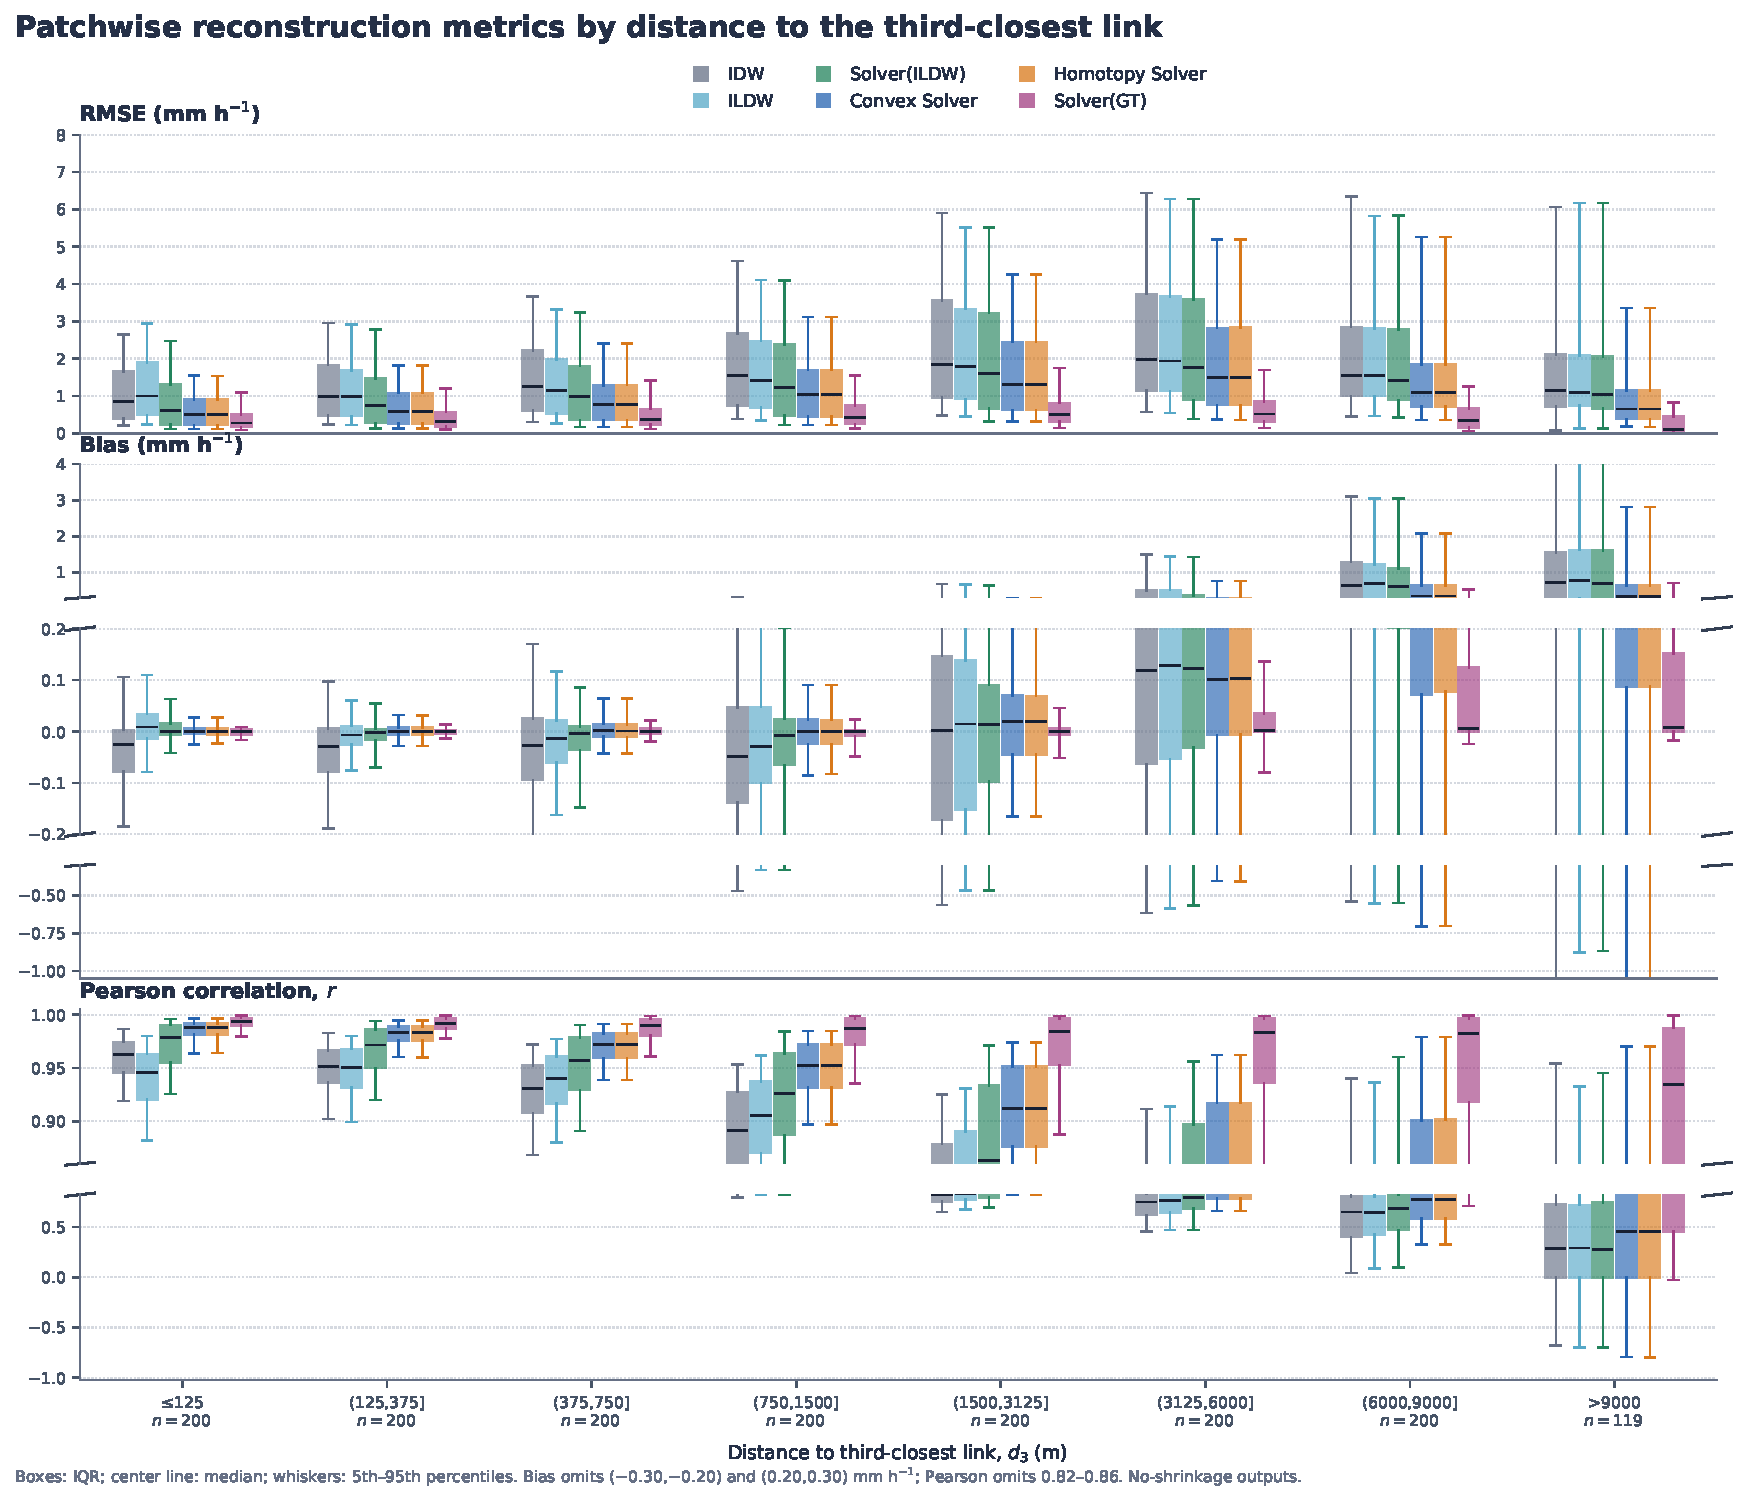
\includegraphics[width=\textwidth]{Journal_200patches_assets_oct21/images/d3_metrics_200_noshrinkage/d3_rmse_bias_pearson_boxplots_200_broken_y.pdf}
  \caption{Box-and-whisker visualization of the $d_3$-stratified reconstruction metrics summarized in Table~\ref{tab:d3-solver-summary}.}
  \label{fig:d3-rmse-bias-pearson-boxplots}
\end{figure}

%%%%%%%%%%%%%%%%%%%%%%%%%%%%%%%%%%%%%%%%%%%%
\section*{Paired $t$ analysis for RMSE}
\Cref{tab:paired-rmse-t-test} summarizes the paired $t$ tests for patchwise RMSE differences relative to \IDW. Negative differences indicate that method A has lower RMSE than \IDW, which is the one-sided alternative tested here. The paired results show lower RMSE than \IDW\ for all alternatives; \ILDW\ wins in 195 of 200 patches, \solverILDW\ wins in 196, and \ConvexSolver\ and \Homotopy\ win in all 200. The mean patchwise RMSE reduction relative to \IDW\ is $0.64$ \si{\milli\meter\per\hour} for both \ConvexSolver\ and \Homotopy\. Table~\ref{tab:paired-rmse-t-test} reports the full paired comparisons.


\begin{table}[H]\centering\scriptsize\setlength{\tabcolsep}{3pt}\resizebox{\textwidth}{!}{\begin{tabular}{lrrrrrrrrrrl}
\toprule
Comparison & $n$ & wins A:\IDW & mean A & mean \IDW & mean diff & SD diff & SE & $t$ & one-sided $p$ & 99\% upper bound & decision \\
\midrule
\ILDW - \IDW & 200 & 195:5 & 2.07 & 2.18 & -0.10 & 0.09 & 0.01 & -15.83 & $2.33 \times 10^{-37}$ & -0.09 & reject \\
\solverILDW - \IDW & 200 & 196:4 & 1.94 & 2.18 & -0.23 & 0.18 & 0.01 & -17.93 & $1.00 \times 10^{-43}$ & -0.20 & reject \\
\ConvexSolver - \IDW & 200 & 200:0 & 1.53 & 2.18 & -0.64 & 0.48 & 0.03 & -19.09 & $3.71 \times 10^{-47}$ & -0.56 & reject \\
\Homotopy - \IDW & 200 & 200:0 & 1.53 & 2.18 & -0.64 & 0.48 & 0.03 & -19.09 & $3.79 \times 10^{-47}$ & -0.56 & reject \\
\solverGT - \IDW & 200 & 200:0 & 0.61 & 2.18 & -1.57 & 1.38 & 0.10 & -16.06 & $4.61 \times 10^{-38}$ & -1.34 & reject \\
\bottomrule\end{tabular}}
\caption{One-sided paired $t$ tests of patchwise RMSE differences against \IDW\ across all 200 patches. Negative differences favor method A; upper bounds are one-sided 99\% bounds.}
\label{tab:paired-rmse-t-test}
\end{table}
%%%%%%%%%%%%%%%%%%%%%%%%%%%%%%%%%%%%%%%

\section*{Paired $t$ analysis for absolute bias}

\Cref{tab:paired-absolute-bias-test} summarizes the paired mean tests for patchwise absolute-bias differences relative to \IDW. Negative differences indicate that method A is closer to zero bias than \IDW, which is the one-sided alternative tested here. The paired results show that all alternatives significantly reduce absolute bias relative to \IDW. The reduction is heterogeneous across patches: \ConvexSolver\ and \Homotopy\ have smaller absolute bias than \IDW\ in 159 of 200 patches, reducing mean absolute bias from $0.21$ to about $0.09$ \si{\milli\meter\per\hour}. Table~\ref{tab:paired-absolute-bias-test} reports the paired comparisons.

%Most importantly, the $99\%$ one-sided upper confidence bound for \ConvexSolver\ is $-0.06$ \si{\milli\meter\per\hour}. Thus, even under this conservative bound, the mean patchwise reduction in absolute bias relative to \IDW\ is at least $0.06$ \si{\milli\meter\per\hour}.

\begin{table}[H]\centering\scriptsize\setlength{\tabcolsep}{3pt}\resizebox{\textwidth}{!}{\begin{tabular}{lrrrrrrrrrrl}
\toprule
Comparison & $n$ & wins A:\IDW & mean A & mean \IDW & mean diff & SD diff & SE & $t$ & one-sided $p$ & 99\% upper bound & decision \\
\midrule
\ILDW - \IDW & 200 & 138:62 & 0.19 & 0.21 & -0.02 & 0.05 & 0.00 & -6.59 & $1.91 \times 10^{-10}$ & -0.02 & reject \\
\solverILDW - \IDW & 200 & 149:51 & 0.17 & 0.21 & -0.05 & 0.09 & 0.01 & -7.32 & $2.91 \times 10^{-12}$ & -0.03 & reject \\
\ConvexSolver - \IDW & 200 & 159:41 & 0.09 & 0.21 & -0.12 & 0.20 & 0.01 & -8.90 & $1.75 \times 10^{-16}$ & -0.09 & reject \\
\Homotopy - \IDW & 200 & 159:41 & 0.09 & 0.21 & -0.13 & 0.20 & 0.01 & -8.91 & $1.62 \times 10^{-16}$ & -0.09 & reject \\
\solverGT - \IDW & 200 & 183:17 & 0.01 & 0.21 & -0.20 & 0.25 & 0.02 & -11.49 & $4.53 \times 10^{-24}$ & -0.16 & reject \\
\bottomrule\end{tabular}}
\caption{One-sided paired $t$ tests of patchwise absolute-bias differences against \IDW\ across all 200 patches. Negative differences favor method A.}
\label{tab:paired-absolute-bias-test}
\end{table}
%%%%%%%%%%%%%%%%%%%%%%%%%%%%%%%%%%%%%%
\section*{Paired comparison of Pearson correlation}

\Cref{tab:paired-pearson-sign-test} summarizes patchwise wins for Pearson correlation relative to \IDW, where higher $r$ indicates better spatial agreement with the ground-truth rainfall field.  The results show that all alternatives improve this measure in most patches. The evidence is strongest for \ConvexSolver, \Homotopy, and \solverGT, which have higher $r$ than \IDW\ in all 200 patches; \ILDW\ and \solverILDW\ win in 190 and 194 patches, respectively. This indicates that the optimization-based methods improve not only RMSE and bias, but also the spatial agreement of the reconstructed rainfall fields.

\begin{table}[H]\centering\begin{tabular}{lrr}
\toprule Comparison & wins A:\IDW & $n$ \\
\midrule
\ILDW - \IDW & 190:10 & 200 \\
\solverILDW - \IDW & 194:6 & 200 \\
\ConvexSolver - \IDW & 200:0 & 200 \\
\Homotopy - \IDW & 200:0 & 200 \\
\solverGT - \IDW & 200:0 & 200 \\
\bottomrule\end{tabular}
\caption{Patchwise Pearson correlation wins over IDW across all 200 patches.}
\label{tab:paired-pearson-sign-test}
\end{table}


%%%%%%%%%%%%%%%%%%%%%%%%%%%%%%%%%%%%%%

\subsection{Taylor Diagrams}
The per-solver Taylor diagrams show one point per patch, with summer patches in red and winter patches in blue.
\begin{figure}[!htbp]\centering
\includegraphics[width=\textwidth]{\taylorsixpanel}
\caption{Per-solver Taylor diagrams for the six reconstruction methods, with one point per patch in each panel (winter blue, summer red). The radius is the reconstructed-field standard deviation normalized by the ground-truth standard deviation (ground truth is at radius 1); the angle represents Pearson correlation. Green dashed contours indicate centered RMSE.}
\label{fig:taylor-per-patch}
\end{figure}
% Pooled Taylor summary temporarily omitted:
% \begin{figure}[!htbp]\centering
% \includegraphics[width=0.78\textwidth]{\taylorsummary}
% \caption{Pooled Taylor summary across all 200 patches, with one aggregate point per solver.}
% \label{fig:taylor-summary}
% \end{figure}

\subsection{Confusion Summaries}
\Cref{tab:wet-dry-confusion-merged} summarizes wet/dry classification at the $0.6$ \si{\milli\meter\per\hour} threshold across all 200 patches. By the fraction-of-all-pixels columns, \ConvexSolver\ reduces false-wet pixels from 0.082 for \IDW\ to 0.047, while false-dry pixels change from 0.004 to 0.005. Among dry ground-truth pixels, the false-wet conditional rate falls from 0.488 to 0.307.

\begin{table}[htbp]\centering\scriptsize\setlength{\tabcolsep}{3pt}\resizebox{\textwidth}{!}{\begin{tabular}{lrrrrrrrrr}
\toprule Method & $n$ & \multicolumn{4}{c}{Fraction of all pixels} & \multicolumn{4}{c}{Conditional rate} \\
\cmidrule(lr){3-6}\cmidrule(lr){7-10}
& & True wet & False wet & True dry & False dry & True wet & False wet & True dry & False dry \\
\midrule
\IDW & 200 & 0.799 & 0.082 & 0.116 & 0.004 & 0.994 & 0.488 & 0.442 & 0.006 \\
\ILDW & 200 & 0.798 & 0.076 & 0.122 & 0.004 & 0.994 & 0.456 & 0.474 & 0.006 \\
\solverILDW & 200 & 0.798 & 0.072 & 0.125 & 0.004 & 0.993 & 0.405 & 0.525 & 0.007 \\
\ConvexSolver & 200 & 0.797 & 0.047 & 0.150 & 0.005 & 0.992 & 0.307 & 0.623 & 0.008 \\
\Homotopy & 200 & 0.797 & 0.047 & 0.150 & 0.005 & 0.992 & 0.307 & 0.623 & 0.008 \\
\solverGT & 200 & 0.799 & 0.012 & 0.185 & 0.003 & 0.996 & 0.171 & 0.759 & 0.004 \\
\\
\bottomrule\end{tabular}}
\caption{Patch-averaged wet/dry confusion at the $0.6$ mm/h threshold across all 200 patches. Fraction columns are normalized by each patch's pixel count; conditional TP/FN rates use wet GT pixels and FP/TN rates use dry GT pixels.}
\label{tab:wet-dry-confusion-merged}
\end{table}


%%%%%%%%%%%%%%%%%%%%%%%%%%%%%%%%%%%%%%%
\subsection{Attenuation Error}
\Cref{tab:attenuation-fit-summary} summarizes the error between the ground-truth attenuation and the attenuation reconstructed from the estimated rainfall field using the forward model. The main quantity is attenuation MAE, reported in \si{\deci\bel\per\kilo\meter}. The table also reports the attenuation cost-function term $J_{\mathrm{atten}}$.
For a given patch $P$ and solver $s$, the attenuation MAE per kilometer equals $\frac{1}{|\mathcal{L}_P|}\sum_{\ell \in \mathcal{L}_P} \frac{\left|\hat{A}_{\ell,s} - A_\ell\right|}{|\ell|}$, where $\hat{A}_{\ell,s}$ is the attenuation implied on link $\ell$ by the ITU-R forward model according to the rain-rate solution $\hat{R}_{P,s}$, $A_\ell$ is the ground-truth attenuation, and $|\ell|$ is the link length in kilometers.

Across the 200 patches, \ConvexSolver\ and \Homotopy\ fit the link attenuations more closely than the interpolation baselines; \Homotopy\ has the lowest mean attenuation MAE ($1.4\times10^{-3}$ \si{\deci\bel\per\kilo\meter}). The same ordering is reflected in $J_{\mathrm{atten}}$, as expected because this term is part of the cost function. \inlinenote{GE: discuss the error compared to ITU attenuation per km for various freqs.}


\begin{table}[H]\centering\small\begin{tabular}{lrrr}
\toprule Solver & $n$ & Attenuation MAE (dB/km) & $J_{\mathrm{atten}}$ \\
\midrule
\IDW & 200 & $0.0819\pm0.0551$ & $0.1068\pm0.1508$ \\
\ILDW & 200 & $0.0222\pm0.0158$ & $0.0089\pm0.0169$ \\
\solverILDW & 200 & $0.0046\pm0.0064$ & $0.0007\pm0.0021$ \\
\ConvexSolver & 200 & $0.0021\pm0.0021$ & $0.0001\pm0.0002$ \\
\Homotopy & 200 & $0.0014\pm0.0014$ & $0.0000\pm0.0001$ \\
\bottomrule\end{tabular}
\caption{Patch-averaged attenuation errors across the 200-patch benchmark. Methods are included when a matching winter and summer solver output is available.}
\label{tab:attenuation-fit-summary}
\end{table}

%%%%%%%%%%%

%%%%%%%%%%%%%%%%%%%%%%%%%%%%%%%%%%%%%%%%%%

\subsection{Patchwise reconstruction metrics by distance to links}
To show how reconstruction quality changes with distance from the microwave links, we compute RMSE, normalized RMSE, signed bias, normalized bias, and Pearson correlation over all pixels in each $d_3$ bin for every patch and solver. Each patch contributes one value to a bin when it contains pixels in that bin. Figures~\ref{fig:d3-rmse}--\ref{fig:d3-pearson} show the distributions across contributing patches; Table~\ref{tab:d3-solver-summary} reports the corresponding mean and sample standard deviation. Each plot uses small multiples, with a separate vertical scale for each distance bin, to make within-bin solver differences visible. Normalized errors divide by the mean ground-truth rain rate over the full patch. The dashed lines in the bias plots mark zero.

\clearpage
\begin{figure}[p]
  \centering
  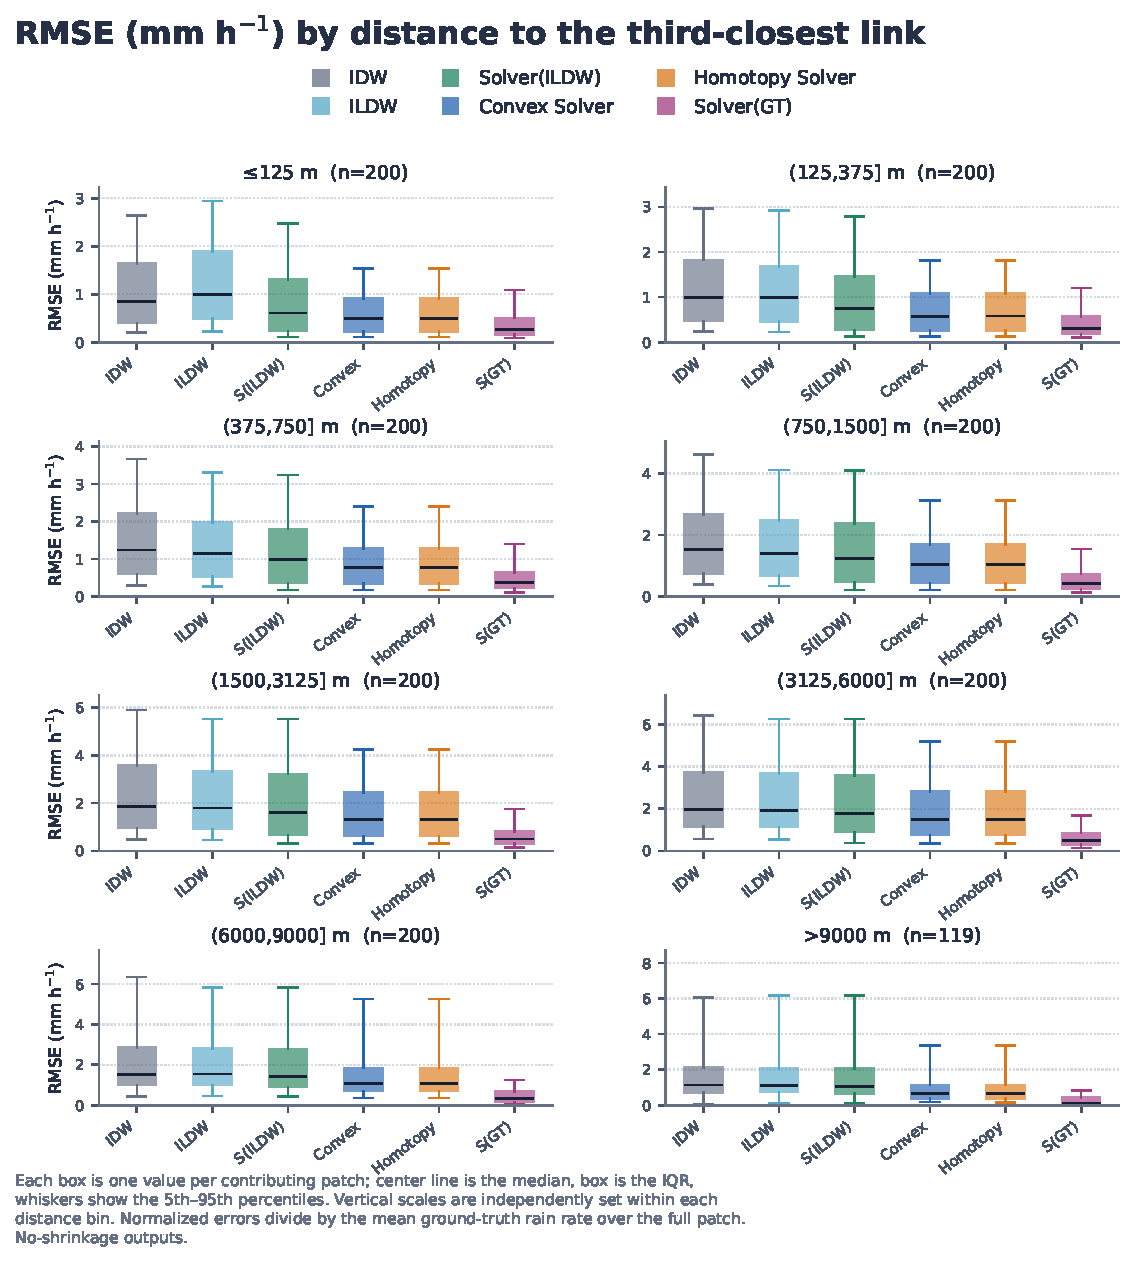
\includegraphics[width=\textwidth,height=.82\textheight,keepaspectratio]{Journal_200patches_assets_oct21/images/d3_metrics_200_noshrinkage/d3_rmse_mm_h_by_bin_200.pdf}
  \caption{Patchwise RMSE by distance to the third-closest link ($d_3$) across the 200-patch benchmark. Each box summarizes values over pixels in the bin for one contributing patch; the center line is the median, the box is the interquartile range, and whiskers span the 5th--95th percentiles. Each panel title gives the number of contributing patches. Vertical scales are independently set by distance bin.}
  \label{fig:d3-rmse}
\end{figure}
\begin{figure}[p]
  \centering
  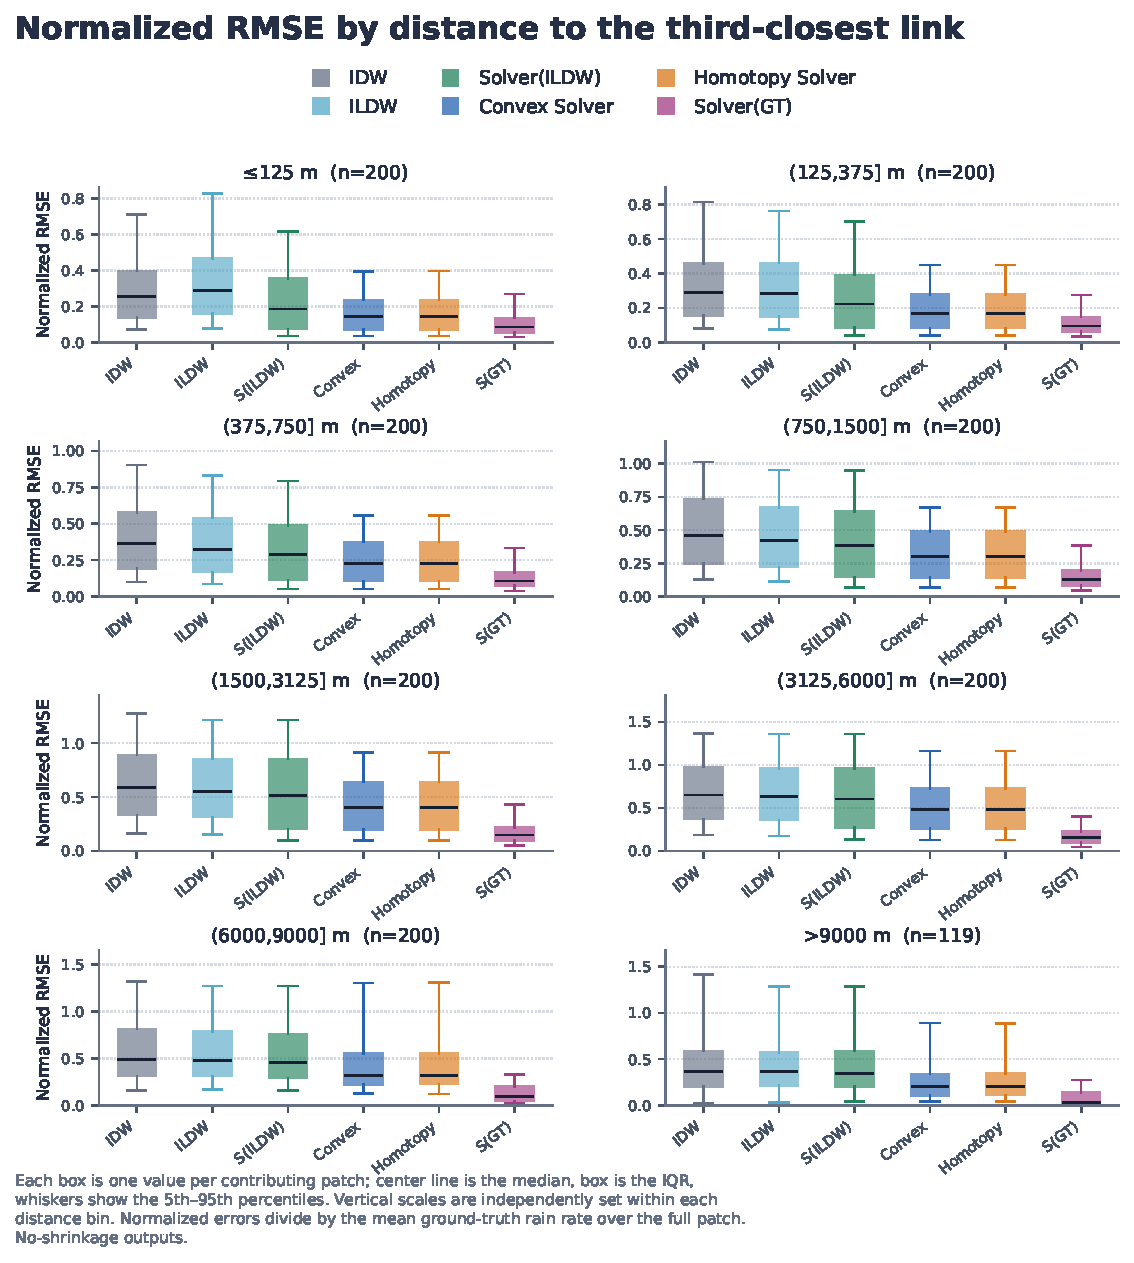
\includegraphics[width=\textwidth,height=.82\textheight,keepaspectratio]{Journal_200patches_assets_oct21/images/d3_metrics_200_noshrinkage/d3_nrmse_by_bin_200.pdf}
  \caption{Patchwise normalized RMSE by distance to the third-closest link ($d_3$). Each patch's RMSE within a distance bin is divided by its mean ground-truth rain rate over the full patch. Boxes and independently scaled panels are defined as in Figure~\ref{fig:d3-rmse}.}
  \label{fig:d3-nrmse}
\end{figure}
\begin{figure}[p]
  \centering
  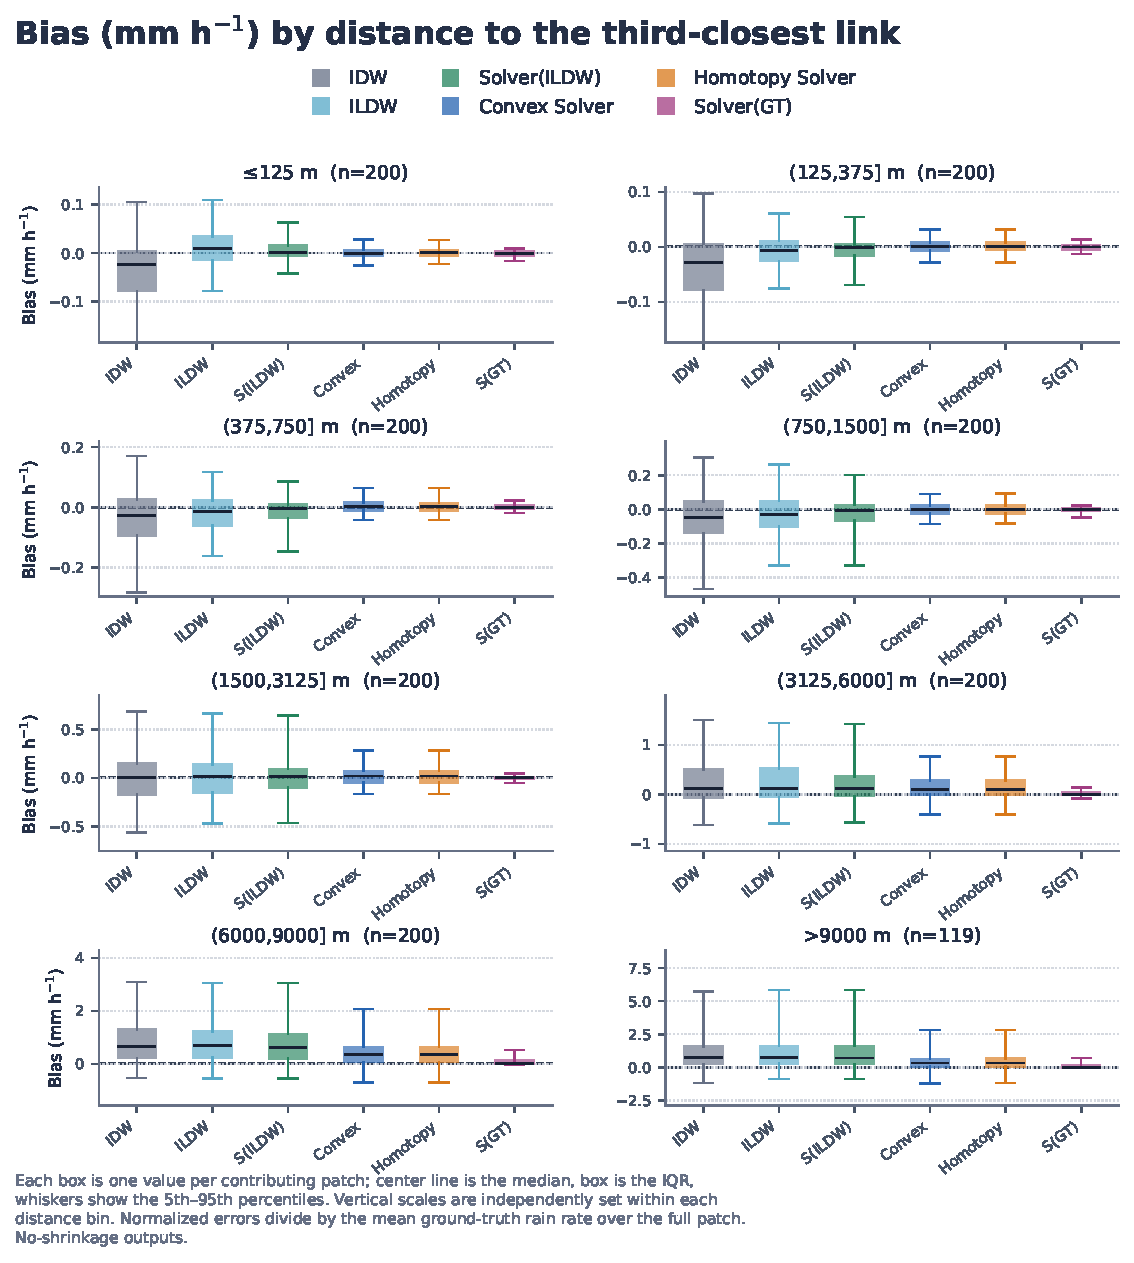
\includegraphics[width=\textwidth,height=.82\textheight,keepaspectratio]{Journal_200patches_assets_oct21/images/d3_metrics_200_noshrinkage/d3_bias_mm_h_by_bin_200.pdf}
  \caption{Patchwise signed bias by distance to the third-closest link ($d_3$), computed as estimated minus ground-truth rain rate within each bin. The dashed line marks zero bias. Boxes and independently scaled panels are defined as in Figure~\ref{fig:d3-rmse}.}
  \label{fig:d3-bias}
\end{figure}
\begin{figure}[p]
  \centering
  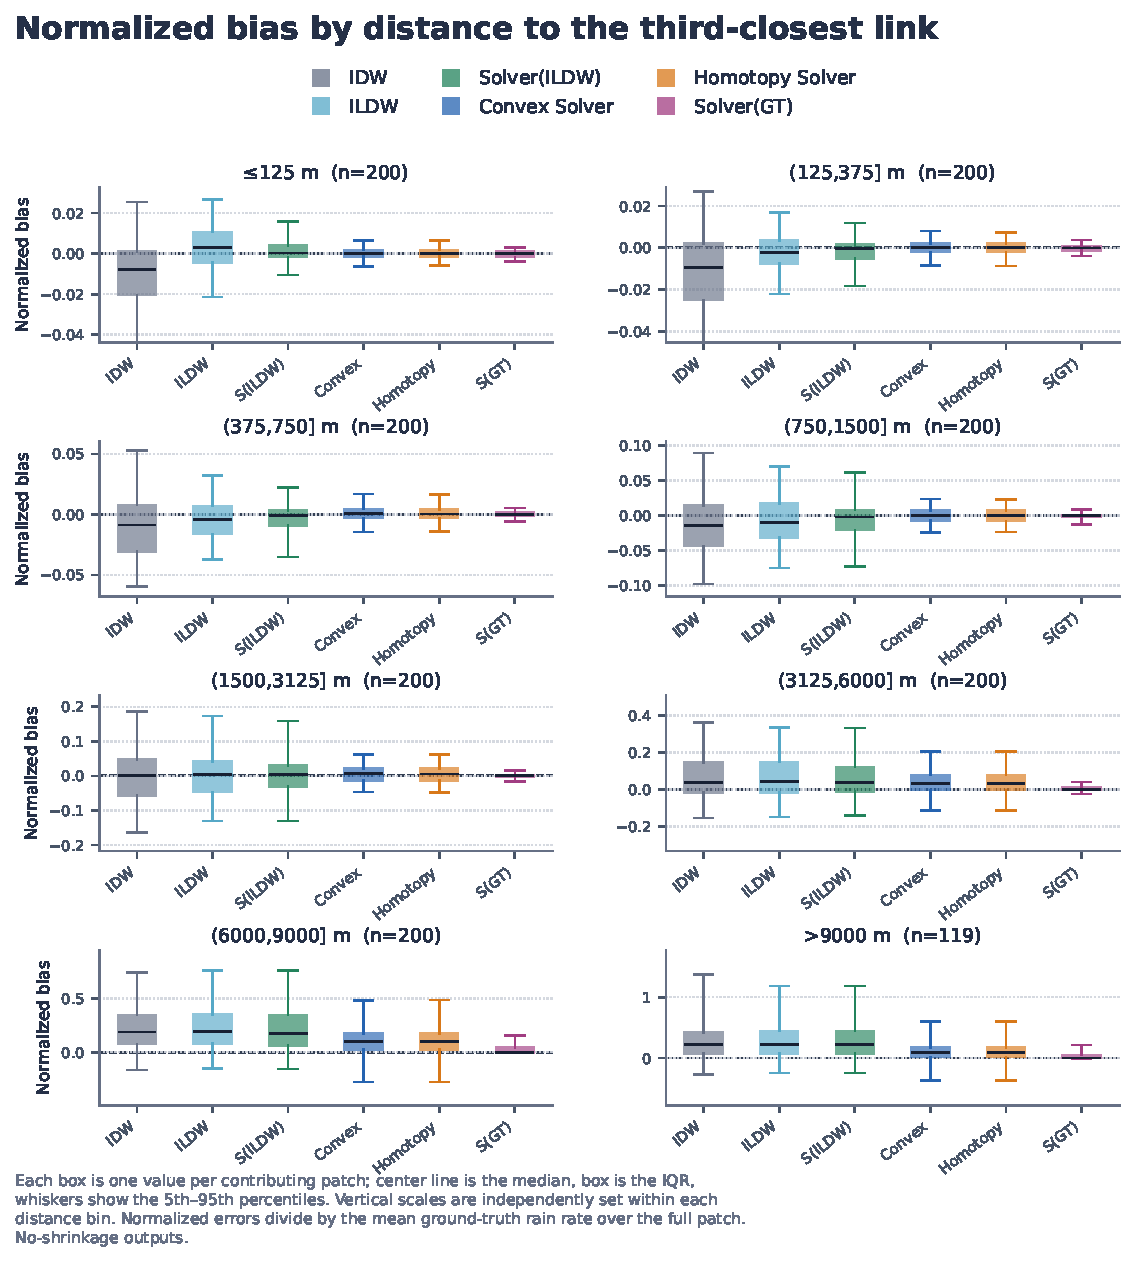
\includegraphics[width=\textwidth,height=.82\textheight,keepaspectratio]{Journal_200patches_assets_oct21/images/d3_metrics_200_noshrinkage/d3_normalized_bias_by_bin_200.pdf}
  \caption{Patchwise normalized signed bias by distance to the third-closest link ($d_3$). Each patch's signed bias within a distance bin is divided by its mean ground-truth rain rate over the full patch. The dashed line marks zero bias. Boxes and independently scaled panels are defined as in Figure~\ref{fig:d3-rmse}.}
  \label{fig:d3-normalized-bias}
\end{figure}
\begin{figure}[p]
  \centering
  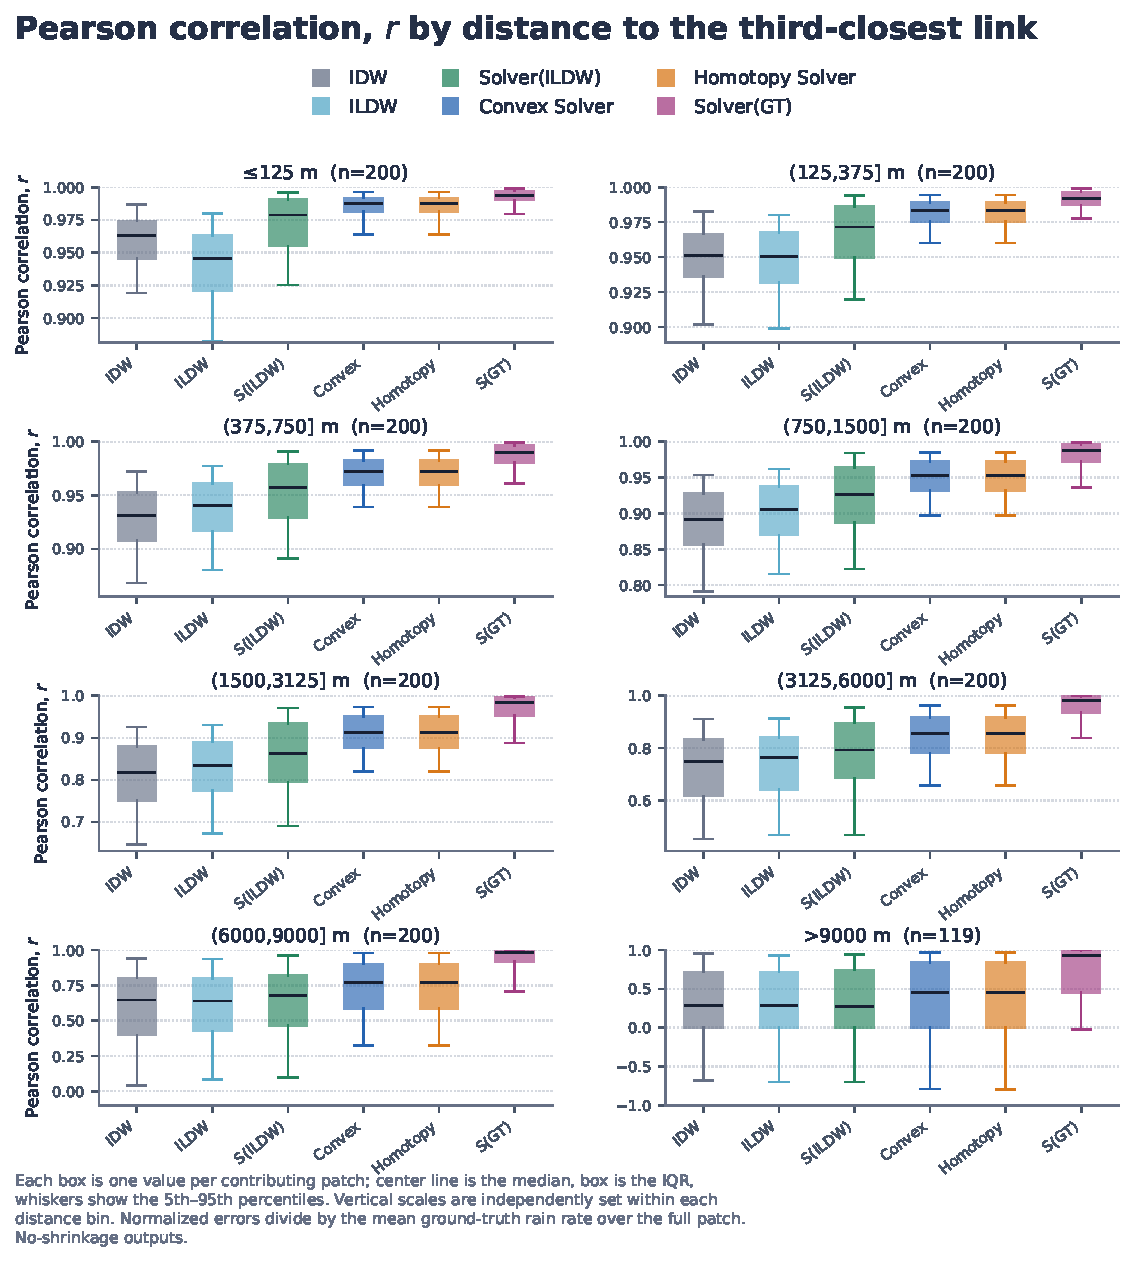
\includegraphics[width=\textwidth,height=.82\textheight,keepaspectratio]{Journal_200patches_assets_oct21/images/d3_metrics_200_noshrinkage/d3_pearson_r_by_bin_200.pdf}
  \caption{Patchwise Pearson correlation by distance to the third-closest link ($d_3$), computed over pixels in each bin. Boxes and independently scaled panels are defined as in Figure~\ref{fig:d3-rmse}.}
  \label{fig:d3-pearson}
\end{figure}
\clearpage



%%%%%%%%%%%%%%%%%%%
%%%%%%%%%%%%%%
%%%%%%%%%
%%%%%
%%%
%


%%%%%%%%%%%%%%%%%%%
%%%%%%%%%%%%%%
%%%%%%%%%
%%%%%
%%%
%
%\input{appendix-case-studies.tex}
\section{Case Study Figures and Objective Evolution}

In this section, we present two case studies, in which we compare  \IDW, \solverGT, and \solverConvex.
In the first case study, \solverGT\ almost equals the ground-truth while \solverConvex\ slightly improves over \IDW.

To quantify how often these two qualitative patterns occur, we use the simple
ratio
\[
q(P)\triangleq
\frac{\mathrm{RMSE}_{P,\ConvexSolver}}
     {\mathrm{RMSE}_{P,\solverGT}}.
\]
We assign patch $P$ to Case~1 (the Case Study~I pattern) when $q(P)\geq2$ and
to Case~2 (the Case Study~II pattern) when $q(P)<2$.  Of the 200 benchmark
patches, 106 are in Case~1 and 94 are in Case~2. The smallest Case~1 ratio
is $2.0041$, whereas the largest Case~2 ratio is $1.9451$; thus no observed
patch lies immediately at the threshold.

For this patch, $J(\solverGT)=1.485$ and RMSE$(\solverGT)=0.102$, while
$J(\ConvexSolver)=0.265$ and RMSE$(\ConvexSolver)=0.703$.
This example shows that a lower value of the objective does not necessarily imply a more accurate reconstruction of the ground-truth rainfall field.
For Case Study I, \Cref{fig:case_gt_convex_202301280900} shows the reconstructed rainfall fields and relative errors, and \Cref{fig:jtrace_gt_convex_202301280900} shows the evolution of the weighted objective over L-BFGS-B iterations.


\begin{figure}[!htbp]
  \centering
  \makebox[\textwidth][c]{\includegraphics[width=1.08\textwidth]{\gtconvexcaseone}}
  \caption{Case Study I: \solverGT\ is visually close to the ground truth. The three upper-right panels show the rainfall fields reconstructed by \IDW, \solverGT, and \solverConvex. The corresponding lower-right panels show the relative error of each reconstruction.}
  \label{fig:case_gt_convex_202301280900}
\end{figure}

\begin{figure}[!htbp]
  \centering
  \begin{minipage}[t]{0.49\textwidth}
    \centering
    \includegraphics[width=\textwidth]{\jgtcaseone}
  \end{minipage}\hfill
  \begin{minipage}[t]{0.49\textwidth}
    \centering
    \includegraphics[width=\textwidth]{\jconvexcaseone}
  \end{minipage}
  \caption{Evolution of the weighted objective over L-BFGS-B  iterations for Case Study I. Left: \solverGT, initialized from the ground-truth field, converges to final $J=1.485$. Right: \ConvexSolver\ reaches a lower final weighted objective, $J=0.265$, but its reconstruction is farther from the ground truth by RMSE.}
  \label{fig:jtrace_gt_convex_202301280900}
\end{figure}
%%%%%%%%%%%%%%
In the second case study, \solverGT\ and \solverConvex\ are visually similar in the reconstruction panels.
For this patch, $J(\solverGT)=0.290$ and RMSE$(\solverGT)=0.536$, while
$J(\ConvexSolver)=0.290$ and RMSE$(\ConvexSolver)=0.559$.
This example shows a case in which the two solutions have almost the same objective value and almost the same reconstruction error.
For Case Study II, \Cref{fig:case_gt_convex_202301310900} shows the reconstructed rainfall fields and relative errors, and \Cref{fig:jtrace_gt_convex_202301310900} shows the evolution of the weighted objective over L-BFGS-B iterations.

\begin{figure}[!htbp]
  \centering
  \makebox[\textwidth][c]{\includegraphics[width=1.08\textwidth]{\gtconvexcasetwo}}
  \caption{Case Study II: \solverGT\ and \solverConvex\ produce visually similar reconstructions. The three upper-right panels show the rainfall fields reconstructed by \IDW, \solverGT, and \solverConvex. The corresponding lower-right panels show the relative error of each reconstruction.}
  \label{fig:case_gt_convex_202301310900}
\end{figure}

\begin{figure}[!htbp]
  \centering
  \begin{minipage}[t]{0.49\textwidth}
    \centering
    \includegraphics[width=\textwidth]{\jgtcasetwo}
  \end{minipage}\hfill
  \begin{minipage}[t]{0.49\textwidth}
    \centering
    \includegraphics[width=\textwidth]{\jconvexcasetwo}
  \end{minipage}
  \caption{Evolution of the weighted objective over L-BFGS-B iterations for Case Study II. Left: \solverGT, initialized from the ground-truth field, converges to final $J=0.290$. Right: \ConvexSolver\ reaches a very similar final weighted objective, $J=0.290$, and a similar RMSE.}
  \label{fig:jtrace_gt_convex_202301310900}
\end{figure}

%%%%%%%%%%%%%%%%%%%%%%%%%%%%%%%%%%%%%%%%%%%%%%%%%%%%%
\section{Discussion}
The benchmark isolates the geometric inversion problem and thereby provides a clear setting for method development. At the same time, several sources of uncertainty remain outside the scope of the current construction, including wet-antenna effects, baseline estimation, quantization, mixed-phase precipitation, and temporal dynamics. These factors matter in operational deployments and should be incorporated in later stages once the benchmarked inverse methods are well understood.

The proposed framework also offers interpretability advantages over purely data-driven alternatives. Because the objective function makes the tradeoff between attenuation consistency, spatial smoothness, and rainfall shrinkage explicit, the resulting reconstructions can be inspected and explained in terms of physically meaningful quantities. In the no-shrinkage results reported here, the rainfall-shrinkage weight is set to zero.


The resulting optimization problem is nonconvex due to the nonlinear attenuation model. We therefore compute a locally optimal solution using L-BFGS-B, initialized from the ILDW estimate. In practice, the combination of strong data constraints and regularization yields stable and consistent reconstructions across instances.

The results highlight the importance of the initialization for the nonconvex optimization procedure. In many instances, the ILDW solution lies close to a stationary point of the objective, and the optimizer produces only marginal changes. This indicates that ILDW already achieves a strong balance between attenuation consistency and spatial regularity. Consequently, the role of the nonconvex optimization is primarily to refine the estimate in instances where these objectives are in stronger conflict. In contrast, IDW provides a weaker initialization due to its simplified geometric representation of links, leading to larger discrepancies with the attenuation model.
%%%%%%%%%%%%%%%%%%%%%%%%%%%%%%%%%%%%%%%%%%%%%%%%%%%%%
\section{Conclusion}
This journal draft integrates a benchmark-oriented view of rainfall reconstruction from commercial microwave links. Starting from hourly EURADCLIM maps, we extract rain events, simulate CML attenuations through a forward model, and evaluate inverse reconstruction methods against known ground truth. The resulting setup reframes rainfall reconstruction from opportunistic sensing networks as a well-posed inverse problem with an explicit and interpretable objective.

\bibliographystyle{plainnat}
%\nocite{*}
\bibliography{Journal_200patches_assets_oct21/references,Journal_200patches_assets_oct21/mybibCML}
\appendix
\crefalias{section}{appendix}

\section{Illustrative Examples}

This appendix presents a minimal example that isolates an important property of the inverse problem. Namely, we give a concrete counterexample showing that $J_{\text{atten}}$ is nonconvex.

\subsection{A $3\times3$ Counterexample to Convexity}
\label{appendix:nonconvexity-example}
Consider one horizontal link $\ell$ crossing the three middle-row pixels of a
$3\times3$ grid.  The crossed length is $0.125$~km in each pixel, so
$|\ell|=0.375$~km.  Let the link use horizontal polarization at
$38.003$~GHz, for which the ITU-R coefficients used here are
$\kappa=0.400171594750$ and $\alpha=0.881535333268$.  For this one-link
instance,
\[
\widehat A(R)=\sum_{p\in\ell}d_p\kappa R(p)^\alpha,
\qquad
J_{\mathrm{atten}}(R)=
\frac{\bigl(\widehat A(R)-A_{\mathrm{obs}}\bigr)^2}{|\ell|}.
\]

Take the two strictly positive fields
\[
R^{(L)}=\begin{bmatrix}1&1&1\\20&1&1\\1&1&1\end{bmatrix},
\qquad
R^{(R)}=\begin{bmatrix}1&1&1\\1&1&20\\1&1&1\end{bmatrix}
\quad \si{\milli\meter\per\hour}.
\]
They are left-right reflections across the grid's vertical centerline.  Either
field could be the ground truth: the link crosses the reflected pixels over
equal lengths, so both fields produce
\[
\widehat A\bigl(R^{(L)}\bigr)=\widehat A\bigl(R^{(R)}\bigr)
=A_{\mathrm{obs}}=0.801595407171\ \si{\deci\bel},
\]
and hence
$J_{\mathrm{atten}}(R^{(L)})=J_{\mathrm{atten}}(R^{(R)})=0$.
Their arithmetic mean is
\[
R^{(M)}=\frac{R^{(L)}+R^{(R)}}{2}
=\begin{bmatrix}1&1&1\\10.5&1&10.5\\1&1&1\end{bmatrix}.
\]
For $g(r)=r^\alpha$, we have
$g''(r)=\alpha(\alpha-1)r^{\alpha-2}<0$ because $0<\alpha<1$; hence $g$ is
strictly concave and
$2(10.5)^\alpha>20^\alpha+1$.  Consequently,
\[
\widehat A(R^{(M)})=0.845082934781\ \si{\deci\bel}>A_{\mathrm{obs}},
\qquad
J_{\mathrm{atten}}(R^{(M)})=0.005043106820>0.
\]
Therefore,
\[
J_{\mathrm{atten}}\!\left(\frac{R^{(L)}+R^{(R)}}{2}\right)
>
\frac{J_{\mathrm{atten}}(R^{(L)})+J_{\mathrm{atten}}(R^{(R)})}{2}=0,
\]
which violates the defining inequality for a convex function.

\end{document}
